\documentclass{elsarticle}
\usepackage{CJK}
\usepackage{rotating}
\usepackage{natbib}
\usepackage{multirow}
\usepackage{amsmath}
\usepackage{amssymb}
\usepackage{latexsym}
\usepackage{threeparttable}
\usepackage{algorithm}
\usepackage{algorithmic}
\usepackage{array}
\usepackage{graphicx}
\usepackage{epsfig}
\usepackage{subfigure}
\usepackage{epstopdf}
\usepackage{url}
\newtheorem{thm}{Theorem}
\newtheorem{property}{Property}
\newtheorem{example}{Example}
\newtheorem{proposition}{Proposition}
\newtheorem{lem}{Lemma}
\newtheorem{rem}{Remark}
\newtheorem{corollary}{Corollary}
\newtheorem{problem}{Problem}
\newproof{proof}{Proof}
\newdefinition{definition}{Definition}
\journal{Pattern Recognition}

\begin{document}

\begin{frontmatter}

% Title, authors and addresses

% use the thanksref command within \title, \author or \address for footnotes;
% use the corauthref command within \author for corresponding author footnotes;
% use the ead command for the email address,
% and the form \ead[url] for the home page:
\title{Frequent pattern discovery with tri-partition alphabets}
%\author{Double blind review}

\author[1]{Fan Min}
\author[2,1]{Zhi-Heng Zhang}
\author[1]{Wen-Jie Zhai}
\author[1]{Rong-Ping Shen}

\address[1]{School of Computer Science, Southwest Petroleum University, Chengdu 610500, China}
\address[2]{School of Science, Southwest Petroleum University, Chengdu 610500, China}

\cortext[cor1]{Corresponding author. Tel.: +86 135 4068 5200.\\ Email: minfanphd@163.com.}

\begin{abstract}
The concept of patterns is the basis of sequence analysis.
There are various definitions of patterns in Biological data, text and time series analysis.
Inspired by the protein tri-partition and three-way decision (3WD), we propose here a frequent pattern discovery algorithm for a new type of pattern by dividing the alphabet into strong/medium/weak parts.
The pattern is more general and flexible than existing ones and is therefore more interesting in applications.
Experiments are undertaken on data in various fields including protein sequences mining, stock price time series analysis, and faked Chinese text keywords mining.
The results show that tri-patterns are more meaningful and desirable than the existing four types.
This study enriches the semantics of sequential pattern discovery and the application fields of 3WD.
\end{abstract}

\begin{keyword}
Pattern discovery; Sequence; Tri-pattern; Tri-wildcard.
\end{keyword}
\end{frontmatter}

\section{Introduction}\label{section: Introduction}
Pattern discovery has been widely studied in machine learning, such as image recognition \cite{Khotanzad1990Invariant} and text analysis \cite{Tausczik2010The}.
A sequential pattern \cite{dietterich1985discovering} is a (totally or partially ordered) subsequence of a transactional dataset \cite{Agrawal1995Mining}, a symbolic sequence \cite{She2003Frequent}, a numeric time series \cite{olominu2014application}, etc.
Sequential pattern discovery (also called pattern mining) \cite{Agrawal1995Mining,Wu2014Pattern} refers to discovering all frequent sequential patterns from these data.
For transactional datasets such as retailing/market-basket and planning \cite{huang2012mining}, a pattern is a sequence of events, where each event is represented by an itemset.
This kind of pattern has the ability to extend both horizontally and vertically, and therefore producing general association rules.
For symbolic sequences such as protein \cite{needleman1970general} and text \cite{Mueen2009Exact}, a pattern is a subsequence of characters, also called a string.
It is simple however meaningful to represent codons \cite{mooney2013sequential} or keywords.
For numeric time series such as stock price \cite{ng2003mining} and petroleum production \cite{olominu2014application}, where the trend of fluctuation is essential to stock holders and the petroleum cooperation, a pattern is a subsequence of real values.

One interesting research direction of symbolic sequential pattern discovery involves the generalization of patterns.
A plain pattern is a subsequence that should be exactly matched.
A wildcard \cite{Chen2006Efficient}, which is also called a motif \cite{Lin2002finding,Wu2015Strict}, matches any character in the alphabet.
Consequently, a wildcard gap \cite{Chen2006Efficient} matches any subsequence within the length constraint.
In this way, a pattern with wildcard gaps is able to handle the noise or shift \cite{yang2002mining}.
To enrich the semantics of the pattern, the alphabet is divided into the weak and strong parts.
A weak-wildcard gap \cite{tanmin2016weak} matches a subsequence of weak characters.
Consequently, a pattern with weak-wildcard gaps \cite{tanmin2016weak} not only ignores weak characters, but also maintains strong ones.

In this paper, we introduce a more general and flexible type called tri-pattern inspired by 3WD \cite{Yao2012AnOutline}.
The alphabet is partitioned into three parts $\Gamma$, $\Lambda$, and $\Omega$ corresponding to strong, medium, and weak characters, respectively.
In this situation, a tri-wildcard gap $(N, M)$ matches any sequence of medium/weak characters with length between $N$ and $M$.
A tri-pattern is a sequence of strong/medium characters containing periodic tri-wildcard gaps, where periodic indicates that the gaps
between any two adjacent characters are identical.
The idea of tri-partition is widely adopted in applications.
Biologists partition the human amino acid alphabet into essential, conditional essential, and nonessential amino acids \cite{amino-acid}.
Petroleum expert partition the oil production fluctuation into significant, insignificant, and minor change.
Tri-partition of situations and actions \cite{li2017three,miao2007granular,yao2013granular} also have attracted much research interests in data mining, especially 3WD \cite{gao2017actionable,HuangB2014Intuitionistic,she2017multiple}.
To the best of our knowledge, however, tri-partition of the alphabet has not been considered in the pattern discovery society.

Tri-patterns are more general than the four existing types.
Let tri-patterns be Type I, plain patterns be Type II, patterns with periodic wildcard gaps \cite{Chen2006Efficient} be Type III, patterns with periodic weak-wildcard gaps \cite{tanmin2016weak} be Type IV, and strong patterns with periodic weak-wildcard gaps \cite{tanmin2016weak} be Type V.
Types II through V are the special cases of Type I on for $\Lambda = \Omega = \emptyset$, $\Lambda = \Sigma$, $\Omega = \emptyset$, and $\Lambda = \emptyset$, respectively.
Similar to existing frequent pattern discovery problems, a new problem for Type I is defined.
With the Apriori property of the new problem, an Apriori algorithm is designed for efficient pattern discovery and tree pruning.

We compare these five types on three application domains to reveal the universality of the new pattern.
The first is the human protein sequence where essential, conditional essential, and nonessential amino acids correspond to strong, medium, and weak characters, respectively.
Twenty sequences are concatenated to mine frequent patterns.
These patterns and their popularity in the original sequences are analyzed.
Tri-patterns are the most meaningful, while other types especially Type II suffer from too many weak characters.
For the pattern popularity, tri-patterns have the best minimal and the second best average performance.

The second is oil well daily production time series.
A coding table is designed to convert the numeric time series into a nominal sequence.
Significant, insignificant, and minor changes correspond to strong, medium, and weak characters, respectively.
The data of an oil well for two years is adopted to mine frequent patterns, which are finally matched in the original time series.
Compared to distance-based approaches that analyze numeric time series directly, the coding and mining approach handles minor difference easier.
Observation on the original time series shows that tri-patterns match some similar subsequences with minor differences.
In contrast, four existing types either excludes some similar subsequences, or includes dissimilar ones.

The third is faked Chinese text.
Notional words, function words, and special characters correspond to strong, medium, and weak characters, respectively.
Four sets of text are collected in news, novel, history, and law.
The background is that some text creators distribute advertisements of illegal stuff such as faked money or invoice.
They may insert some characters into the text, which makes the text still readable but hard for automated analysis.
Our purpose is to extract keywords from the faked text, which are also keywords in the original text.
This problem is closely relevant to text fuzzy matching and keywords extraction.
With tri-patterns, the algorithm obtains the best accuracy in mining the keywords from the faked text.

The remainder of this paper is organized as follows.
Section \ref{section: problem} defines the new type of patterns, analyzes the relationships among five types, and presents the new pattern discovery problem.
Section \ref{section: algorithm-design} demonstrates the Apriori property and proposes the new algorithm.
Section \ref{section: results} explains experimental settings and results on three kinds of real-world data.
Finally, concluding remarks are discussed in Section \ref{section: conclusions}.

\section{Related work}\label{section: related-work}
In this section, we present some related work concerning 3WD and sequential pattern discovery.

\subsection{Three-way decision}\label{subsection: three-way-decision}
In rough set theory \cite{Pawlak1982Rough}, according to the equivalence relation, the universe is partitioned into three disjoint regions.
The positive (negative, boundary) region is the set of objects that are definitely (definitely not, possibly) members of the target set.
However, this strict division often hinders its application in practice.
Probabilistic rough set models such as decision-theoretical rough sets (DTRS) \cite{Xu2016Generalized,Yao1992ADecision} and variable precision rough sets \cite{Ziarko1993Variable} are introduced for this issue.
Among them, DTRS is a sound theory based on Bayesian decision making \cite{Greco2007Bayesian}.
The required parameters are systematically determined based on costs of various decisions \cite{Yao2009Three,Yao1992ADecision}.

3WD has made a big step forward through making itself a methodology of divide and conquer \cite{Yao2016Three} rather than a concrete technique.
With this methodology, one task is to construct a trisection or a tri-partition of the universal set.
The other is to act upon objects in one or more regions by developing appropriate strategies.
3WD is a class of effective ways and heuristics commonly used in human problem solving and information processing.

Recently, various theories are inspired by 3WD.
Three-way formal concept analysis \cite{Sang2017Decision} is constructed with the three-way operators and their inverse.
Three-way cognition computing \cite{li2017three} focuses on concept learning via multi-granularity from the viewpoint of cognition.
Three-way fuzzy sets \cite{Deng2014Decision} constructs a three-way, three-valued, or three-region approximation with a pair of thresholds on the fuzzy membership function.
Three-way decisions space \cite{Hu2014Three} unifies decision measurement, decision conditions and evaluation functions.
Sequential three-way decisions \cite{Li2013Cost} is an iteration process that eventually leads to two-way decisions.
There are also some generalized three-way decision models \cite{Li2017Generalized,liu2016novel}.

There are also various 3WD applications.
Three-way recommender system is applied to both classification \cite{Zhang2016Three} and regression \cite{zhang2017regression} of user ratings.
Three-way active learning \cite{Min2017Tri,WangMinZhangWu2017Active} achieves a tradeoff between teacher cost for acquiring class labels and misclassification costs.
Three-way clustering \cite{Yu2012Three} introduces a new strategy for overlapping clustering based on the DTRS model.
Three-way spam filtering \cite{Bing2014Cost} reduces the email misclassification costs.
Three-way face recognition \cite{Li2016Sequential} develops a sequential strategy to address the imbalanced misclassification cost and insufficient high quality facial image information.

\subsection{Sequential pattern discovery}\label{subsection: pattern-discovery}
The sequence data can be usually categorized according to the elementary data type, namely numeric \cite{Li2016A}, symbol \cite{Vladimir2015Methods} and image \cite{Michael2000Understanding}.
Most of time series such as weather \cite{Li2016A} and stock \cite{Wenbin2015The} are numerical.
However, symbolic sequence data usually contains text \cite{Pletscherfrankild2015DISEASES} and biological data \cite{Vladimir2015Methods}.
Image sequence data are commonly collected from traffic \cite{Michael2000Understanding} and medical videos \cite{Zhu2003Medical}.

The definition of the pattern varies according to the practical problem.
For numeric time series, a pattern is a segment that reveals certain trends \cite{Trottini2015On} or periodicity \cite{Lopes2015Looking}.
The key issue of pattern matching is the similarity model.
For symbolic sequences, a pattern is a subsequence representing keywords \cite{Mihalcea2004TextRank} or associations \cite{Andradeab2000Automated}.
Wildcards \cite{Chen2006Efficient} and fuzzy matching are often used to find more candidates.
For videos, a pattern is part of the images representing vehicles, pedestrians and obstacles for traffic \cite{Alexander2001Robust}, or viscera and mass \cite{Tang2009Digital} for medical image sequence.

Pattern discovery algorithms are designed for different types of data and patterns.
Due to the exponential nature of respective problems, efficiency is the main concern of these algorithms.
For trend and periodicity analysis, various regression analysis methods \cite{Michelle2015Statistics} proposed.
For symbolic sequences pattern mining, Apriori \cite{Agrawal1995Mining} and SPADE \cite{Zaki2001SPADE} algorithms are often employed for efficient pruning.
For image processing, artificial neural network \cite{Lo1995Artificial} and random walk \cite{Kim2015Spatiotemporal} are often employed to handle complex situations.
It is worthy noted that numeric time series are usually converted into symbolic ones \cite{Chiu2003Probabilistic,tanmin2016weak} to facilitate pattern mining.


\section{Problem statement}\label{section: problem}
In this section, we first propose a general type of pattern which will be called tri-patterns.
Second we discuss the frequency of tri-pattern.
Third we analyze its relationships with four existing types.
Finally we define the problem of frequent tri-pattern discovery.
Table \ref{table: Notation} lists notations used throughout the paper.
\begin{table}[htb]\caption{Notations}\label{table: Notation}
\centering
\setlength{\tabcolsep}{8pt}
\begin{tabular}{lll}
\hline
Notation                & Meaning                                                    \\
\hline
$\Sigma$                & An alphabet  \\
$T = (\Gamma, \Lambda, \Omega)$ & The strategy of tri-partition\\
$\Gamma$                & The set of strong characters  \\
$\Lambda$               & The set of medium characters\\
$\Omega$                & The set of weak characters       \\
$S$                     & A sequence                     \\
$k$                     & The length of $S$ \\
$sub(S, i, j)$          & A sub-sequence of $S$ from position $i$ to $j$\\
$N$                     & The gap lower bound             \\
$M$                     & The gap upper bound             \\
$\psi$               & A tri-wildcard for $P$ \\
$P$                     & A tri-pattern                      \\
$m$                     & The length of $P$  \\
$w(N, M) = (N, M)$                & The tri-wildcard gap for $P$                    \\
$sub(P, I) $            & A sub-pattern of $P$ on $I$\\
$\mathcal{P}$           & The set of all tri-patterns      \\
$\mathcal{P}_i$         & The set of all tri-patterns with length $i$    \\
$I = \langle i_1, i_2, \cdots, i_m \rangle$    & A position sequence\\
$sup(P, S)$             & The number of $I$ which $P$ actually matches $S$\\
$ofs(P, S)$             & The number of $I$ which $P$ probably matches $S$\\
$fr(P, S)$               & The frequency of $P$, which is $\frac{sup(P, S)}{ofs(P, S)}$\\
$\rho$                  & The user-specified frequency threshold  \\
\hline
\end{tabular}
\end{table}

\subsection{Tri-patterns}\label{subsection: tri-patterns}
The starting point of sequential pattern discovery is an alphabet, which is fundamental in both natural and formal languages.
\begin{definition}\label{definition: alphabet}
An \textbf{alphabet} $\Sigma$ is a non-empty finite set, whose elements are called \textbf{characters}.
\end{definition}

According to the $\Sigma$, a sequence can be defined as a series of ordered characters.
\begin{definition}\label{definition: sequence}
Any $S = s_1 s_2 \dots s_k$ where $s_i \in \Sigma$ for any $1 \leq i \leq k$ is a \textbf{sequence}, which is also called a string.
The length of the sequence is $|S| = k$.
\end{definition}

For example, $\Sigma$ = \{o, a, b, c\} is an alphabet, $S$ = aboacbb is a sequence on the alphabet, and $|S| = 7$.

One contribution of this work is to partition the alphabet into three disjoint subsets, which are enriched with certain semantics respectively.
\begin{definition}\label{definition: triple-alphabet}
$T = (\Gamma, \Lambda, \Omega)$ where $\Sigma = \Gamma \cup \Lambda \cup \Omega$ and $\Gamma \cap \Lambda$ = $\Gamma \cap \Omega$ = $\Lambda \cap \Omega = \emptyset$ is a tri-partition of $\Sigma$.
$\Gamma$ is the set of \textbf{strong characters}, $\Lambda$ is the set of \textbf{medium characters}, and $\Omega$ is the set of \textbf{weak characters}.
\end{definition}

This partition strategy $T = (\Gamma, \Lambda, \Omega)$ is used in two ways.
One is the definition of the tri-wildcard.
\begin{definition}\label{definition: tri-wildcard}
A tri-wildcard $\psi$ is a symbol that matches any character in $\Lambda \cup \Omega$.
A \textbf{tri-wildcard gap} $w(N, M)$ is a sequence of tri-wildcards with minimal size $N$ and maximal size $M$.
\end{definition}

\begin{example}\label{example: tri-wildcard-gap}
Let $\Sigma$ = \{o, a, b, c\}, $\Gamma$ = \{c\}, $\Lambda$ = \{a, b\}, and $\Omega$ = \{o\}.
$\psi$ matches a, b, o except c.
The gap with size 2 ($M - N + 1 = 2$) matches a, ab, aa, etc, but not ca, oaa, etc.
Gap $w(N, M)$ is also denoted by $(N, M)$ in a pattern.
\end{example}

The other is the definition of tri-pattern.
\begin{definition}\label{definition: weak-pattern}
A \textbf{tri-pattern} (Type I pattern) is a sequence of strong/medium characters and periodic tri-wildcard gaps that begins and ends with tri-wildcards matching medium or weak characters.
It has the following form:
\begin{equation}
P = p_1(N, M)p_2(N, M)\dots(N, M)p_m,
\end{equation}
where $m$ is the length of the pattern, $p_i \in \Gamma \cup \Lambda$ for any $1 \leq i \leq m$.
\end{definition}

Moreover, the tri-wildcard gap $(N, M)$ is the position constraint for each $p_i$, $i \in [2, m]$.
Namely, for each pair $p_i(N, M)p_{i+1}$, $1 \leq i \leq m$, the nearest distance is $N$, and the furthest is $M$.
When $N$ and $M$ is known, the pattern is also denoted as $P = p_1p_2\dots p_m$ for brevity.

\begin{example}\label{example: tri-pattern}
Let $\Sigma$, $\Gamma$, $\Lambda$ and $\Omega$ be the same as Example \ref{example: tri-wildcard-gap}.
$P_1 =$ a(0,1)c(0,1)b = acb is a valid pattern.
$P_2 =$ a(0,1)o(0,1)b = aob is an invalid pattern because $p_2 =$ o $\not\in \Gamma \cup \Lambda$.
\end{example}

\begin{figure}[htb]
   \centering
	   \includegraphics[width=2.5in]{tri-partition-and-thier-actions.pdf}
\caption{Tri-partition strategies and actions.}
\label{figure: Tri-partition-strategies-and-actions}
\end{figure}

Figure \ref{figure: Tri-partition-strategies-and-actions} shows the three different actions for respective kinds of characters defined by Definition \ref{definition: triple-alphabet}.
The strong elements of $\Gamma$ are only used to form the characters $p_i$ of tri-pattern.
The weak characters of $\Omega$ are only used to match the tri-wildcard $\psi$.
The medium characters of $\Lambda$ not only can be used to form the characters $p_i$ of tri-pattern, but also can be used to match the tri-wildcard.

\subsection{Frequency}\label{subsection: Frequency}

In order to obtain the frequency of tri-pattern $P$, we first adopt the definition in \cite{min2012apriori} as follows.
\begin{definition}\label{definition: offset-sequence}\cite{min2012apriori}
Given a sequence $S$ with length $k$, gap lower bound $N$ and upper bound $M$,
an offset sequence $I = \langle i_1, i_2, \dots, i_m \rangle$ is a \textbf{position sequence} iff
\begin{enumerate}[1)]
\item{$1 \leq i_1 \leq k$; and}
\item{$N \leq i_{j + 1} - i_j - 1 \leq M$ for all $1 \leq j \leq m - 1$.}
\end{enumerate}
\end{definition}

Consequently, the following proposition holds.
\begin{proposition}\label{proposition: ofs}\cite{min2012apriori}
Let $S = s_1 s_2 \dots s_k$ and $P = p_1(N, M)p_2(N, M)\dots$ $(N, M)p_m$, the number of all position sequences is
\begin{equation}
ofs(P, S) = k (M - N + 1)^{m - 1}.
\end{equation}
\end{proposition}

The key issue is how the tri-pattern matches the sequence.
\begin{definition}\label{definition: weak-occurrence}
Let $S = s_1 s_2 \dots s_k$ be a sequence and $P = p_1(N, M)p_2(N, M)\dots$ $(N, M)p_m$ be a tri-pattern.
If there exists a position sequence $I = \langle i_1, i_2, \dots, i_m\rangle$ so that
\begin{enumerate}[1)]
\item{$1 \leq i_1 < i_2 < \cdots < i_m \leq k$;}
\item{$s_{i_j} = p_j$ for all $1 \le j \le m$;}
\item{$N \le i_{j + 1} - i_j - 1 \le M$ for all $1 \le j \le m - 1$; and}
\item{$\forall i_j < c < i_{j + 1}$ where $1 \le j \le m - 1$, $s_c \in \Lambda \cup \Omega$,}
\end{enumerate}
$I$ is called an \textbf{occurrence} of $P$ in $S$.
\end{definition}

We also say that $P$ matches $S$ at $I$.
The number of occurrences/matches of $P$ in $S$ will be denoted by $sup(P, S, \Gamma, \Lambda, \Omega)$.
It is also called the support of $P$ in $S$.

Finally, we define the frequency of a tri-pattern in a sequence.
\begin{definition}\label{definition: pattern-frequency}
Let $S = s_1 s_2 \dots s_k$ be a sequence and $P = p_1(N, M)p_2(N, M)\dots$ $(N, M)p_m$ be a tri-pattern.
The frequency of $P$ in $S$ is
\begin{equation}\label{equation: pattern-frequency}
fr(P, S, \Gamma, \Lambda, \Omega) = \frac{sup(P, S, \Gamma, \Lambda, \Omega)}{ofs(P, S)}.
\end{equation}
\end{definition}

When $\Gamma$, $\Lambda$, and $\Omega$ are known, $fr(P, S, \Gamma, \Lambda, \Omega)$ and $sup(P, S, \Gamma, \Lambda, \Omega)$ are abbreviated as $fr(P, S)$ and $sup(P, S)$, respectively.
Moreover, we have the following example.

\begin{example}\label{example: pwg-patterns}
Let $\Sigma$ = \{o, a, b, c\}, $\Gamma$ = \{c\}, $\Lambda = \{a, b\}$, $\Omega = \{o\}$, $S$ = acbcbacaocbbba, $N = 0$, $M = 1$, and $P_1 =$ acbb.

$I_1 = \langle 6, 7, 11, 12\rangle$ is not a position sequence because the gap between positions 7 and 11 is 3, which is greater than $M$.
$I_2 = \langle 1, 2, 3, 5\rangle$ is not an occurrence of $P_1$ in $S$ because $s_4 =$ c $\not\in \Lambda \cup \Omega$.
$I_3 = \langle 8, 10, 11, 12\rangle$, $I_4 = \langle 8, 10, 11, 13\rangle$ and $I_5 = \langle 8, 10, 12, 13\rangle$ are three occurrences.

$fr(P_1, S) = \frac{3}{14 \times 2^3} = \frac{3}{112} = 0.0268$.
\end{example}

\subsection{Relationships with existing patterns}\label{subsection: relationship}
There are various definitions of existing patterns.
We list them and discuss their relationships with the tri-pattern (Type I).

\begin{figure}[H]
   \centering
	   \includegraphics[width=3.5in]{relationship.pdf}
\caption{Relationships among different pattern types.}
\label{figure: relationships}
\end{figure}

Plain patterns (Type II pattern) are the simplest type of patterns.
They do not enable any gap between adjacent characters.
Naturally, a plain pattern only permits accurate matching.
\begin{proposition}\label{proposition: plain-pwg}
Type II pattern is a special case of Type I pattern where $N = M = 0$.
\end{proposition}

Wildcard was introduced to obtain certain flexibility.
\begin{definition}\label{definition: wildcard}\cite{Chen2006Efficient}
A wildcard $\phi$ is a special symbol that matches any character in $\Sigma$.
A \textbf{wildcard gap} $g(N, M)$ is a sequence of wildcards of minimal size $N$ and maximal size $M$.
\end{definition}

The concept of pattern with periodic wildcard gaps (Type III pattern) is similar to the Type I pattern.
The only difference is that a Type III pattern employs wildcard gaps instead of weak-wildcard gaps.
It does not need a partition of $\Sigma$ since the wildcard matches any character.
\begin{proposition}\label{proposition: wildcard}
Type III pattern is a special case of Type I pattern where $\Lambda = \Sigma$.
\end{proposition}

Naturally, in this case $\Gamma = \Omega = \emptyset$.

The weak-wildcard gap was introduced in \cite{tanmin2016weak} to control the flexibility of a pattern.
However the concept is slightly different from this work.
To define it, the alphabet is divided into two disjoint subsets, i.e., the set of strong characters $\Gamma$ and the set of medium characters $\Lambda$.
In this case, a tri-wildcard $\varphi$ is a special symbol that matches any character in $\Lambda \subseteq \Sigma$.
In other words, $\varphi$ does not match any character in $\Gamma$.
If we replace wildcard gaps of Type II patterns with weak-wildcard gaps based on $\varphi$, we obtain Type IV patterns.
They are called pattern with periodic weak-wildcard gaps in \cite{tanmin2016weak}.
\begin{proposition}\label{proposition: weak-pattern}
Type IV pattern is a special case of Type I pattern where $\Omega = \emptyset$.
\end{proposition}

Sometimes $\Sigma$ is divided into two disjoint subsets, i.e., the set of strong characters $\Gamma$ and the set of weak characters $\Omega$.
Strong characters can be used to form patterns, while weak characters cannot.
The tri-wildcard $\varphi$ matches any character in $\Omega$.
In this case we have the concept of strong patterns with periodic tri-wildcard gaps (Type V patterns) \cite{tanmin2016weak}.
\begin{proposition}\label{proposition: strong-weak-pattern}
Type V pattern is a special case of Type I pattern where $\Lambda = \emptyset$.
\end{proposition}

The relationships among all five types of patterns are illustrated in Figure \ref{figure: relationships} and listed in Table \ref{table: relationships}.
\begin{table}[tb]\caption{Four special cases of tri-pattern (Type I)}\label{table: relationships}
\centering
\setlength{\tabcolsep}{2pt}
\begin{tabular}{cccccc}
\hline
Type      & Property  &  Statement\\
\hline
II        & $N = M = 0$ & No gap\\
III       & $\Gamma = \Omega = \emptyset$ & $\psi$ matches any character\\
IV        & $\Omega = \emptyset$          & $\psi$ matches any character in $\Lambda$\\
V         & $\Lambda = \emptyset$         & Characters matched by $\psi$ cannot be included in $P$\\
\hline
\end{tabular}
\end{table}

For completeness, one may discuss other three types where $\Gamma = \emptyset$, $\Gamma = \Lambda = \emptyset$, and $\Lambda = \Omega = \emptyset$.
In fact, the case $\Gamma = \Lambda = \emptyset$ is meaningless since no pattern can be formed.
The case $\Lambda = \Omega = \emptyset$ is equivalent to $N = M = 0$ since no wildcard exists.
Hence we will not discuss them further.

\subsection{Proposed problem}\label{subsection: proposed-problem}
Now we propose the pattern discovery problem of tri-pattern.
\begin{problem}\label{problem: frequent-pattern-mining-with-tri-partition-alphabets}
Frequent tri-pattern discovery.\\
\textbf{Input}: $\Sigma$, $\Gamma$, $\Lambda$, $\Omega$, $S$, $\rho$, $N$, $M$.\\
\textbf{Output}: $\mathcal{P}$ = $\mathcal{P}(\Sigma, \Gamma, \Lambda, \Omega, S, \rho, N, M)$.\\
\textbf{Constraint}: any $P \in \mathcal{P}$, $fr(P, S) \geq \rho$.
\end{problem}

$\Sigma$, $\Gamma$, $\Lambda$, $\Omega$, $S$, $N$, $M$ and $P$ have been defined in Definitions \ref{definition: alphabet}-\ref{definition: weak-pattern}.
$\rho$ is the frequent threshold of tri-pattern $P$.
Naturally, $\mathcal{P}$ varies with different parameters.
When $\Lambda$ changes, we have the following property.

\begin{property}\label{property: lambda-eats-gamma}
Let $\Lambda_1 \subset \Lambda_2 \subseteq \Sigma$,
\begin{equation}\label{equation: lambda-subset}
\begin{array}{l}
\mathcal{P}(\Sigma, \Sigma - \Lambda_1 - \Omega, \Lambda_1, \Omega, S, \rho, N, M) \\
\subseteq \mathcal{P}(\Sigma, \Sigma - \Lambda_2 - \Omega, \Lambda_2, \Omega, S, \rho, N, M).
\end{array}
\end{equation}
\end{property}

\begin{proof}
Let $P = p_1p_2 \dots p_m \in$ $\mathcal{P}(\Sigma, \Sigma - \Lambda_1 - \Omega,$ $\Lambda_1, \Omega, S, \rho, N, M).$
Suppose further that $I = \langle i_1, i_2, \dots, i_m\rangle$ is an occurrence of $P$ on $S$ given the tri-partition $T_1 = (\Sigma - \Lambda_1 - \Omega, \Lambda_1, \Omega)$.

Condition (1) According to Definition \ref{definition: weak-pattern}, $\forall 1 \leq i \leq m$, $p_i \in (\Sigma - \Lambda_1 - \Omega) \cup \Lambda_1$
$ = \Sigma - \Omega$ = $(\Sigma - \Lambda_2 - \Omega) \cup \Lambda_2$.

Condition (2) Since $\Lambda_1 \subset \Lambda_2$, $\forall i_j < c < i_{j + 1}$ where $1 \le j \le m - 1$, $s_c \in \Lambda_1 \cup \Omega \subseteq \Lambda_2 \cup \Omega$.

Combining conditions (1)-(2) and Definition \ref{definition: weak-occurrence}, $I$ is also an occurrence of $P$ on $S$ given the tri-partition $T_2 = (\Sigma - \Lambda_2 - \Omega, \Lambda_2, \Omega)$.
Hence $sup(P, S, \Sigma - \Lambda_2 - \Omega, \Lambda_2, \Omega) \geq sup(P, S, \Sigma - \Lambda_1 - \Omega, \Lambda_1, \Omega)$.
Because $ofs(P, S)$ is independent from the alphabet partition, we have $fr(P, S, \Sigma - \Lambda_2 - \Omega, \Lambda_2, \Omega) \geq fr(P, S, \Sigma - \Lambda_1 - \Omega, \Lambda_1, \Omega) \geq \rho$.
Consequently $P \in \mathcal{P}(\Sigma, \Sigma - \Lambda_2 - \Omega, \Lambda_2, \Omega, S, \rho, N, M)$.
Therefore, Equation \eqref{equation: lambda-subset} holds.
\end{proof}

Property \ref{property: lambda-eats-gamma} shows that if we set more strong characters as medium characters, the number of patterns never decrease.
As an extreme case, we have the following corollary:
\begin{corollary}\label{corollary: lambda-empty}
\begin{equation}\label{equation: lambda-emptyset}
\begin{array}{l}
\mathcal{P}(\Sigma, \Sigma - \Omega, \emptyset, \Omega, S, \rho, N, M) \\
\subseteq \mathcal{P}(\Sigma, \Sigma - \Lambda - \Omega, \Lambda, \Omega, S, \rho, N, M).
\end{array}
\end{equation}
\end{corollary}

According to Proposition \ref{proposition: strong-weak-pattern}, Type V pattern is a special case of Type I patterns where $\Lambda = \emptyset$.
Corollary \ref{corollary: lambda-empty} shows that there are more Type I patterns than Type V ones.

Now we look at how the number of patterns changes w.r.t. the change of $\Omega$.
\begin{property}\label{property: omega-eats-lambda}
Let $\Omega_1 \subset \Omega_2 \subseteq \Sigma$,
\begin{equation}\label{equation: omega-subset}
\begin{array}{l}
\mathcal{P}(\Sigma, \Gamma, \Sigma - \Gamma - \Omega_1, \Omega_1, S, \rho, N, M) \\
\supseteq \mathcal{P}(\Sigma, \Gamma, \Sigma - \Gamma - \Omega_2, \Omega_2, S, \rho, N, M).
\end{array}
\end{equation}
\end{property}

\begin{proof}
Let $P = p_1p_2 \dots p_m \in$ $\mathcal{P}(\Sigma, \Gamma, \Sigma - \Gamma - \Omega_2, \Omega_2, S, \rho, N, M)$.
Suppose further that $I = \langle i_1, i_2, \dots, i_m\rangle$ is an occurrence of $P$ on $S$ given the tri-partition $T_2 = (\Gamma, \Sigma - \Gamma - \Omega_2, \Omega_2)$.

Condition (1) According to Definition \ref{definition: weak-pattern}, $\forall 1 \leq i \leq m$, $p_i \in \Gamma \cup (\Sigma - \Gamma - \Omega_2)$
$ = \Sigma - \Omega_2$ $\subset$ $\Sigma - \Omega_1$ = $\Gamma \cup (\Sigma - \Gamma - \Omega_1)$.

Condition (2) $\forall i_j < c < i_{j + 1}$ where $1 \le j \le m - 1$, $s_c \in (\Sigma - \Gamma - \Omega_2) \cup \Omega_2 = \Sigma - \Gamma = (\Sigma - \Gamma - \Omega_1) \cup \Omega_1$.

Combining conditions (1)-(2) and Definition \ref{definition: weak-occurrence}, $I$ is also an occurrence of $P$ on $S$ given the tri-partition $T_1 = (\Gamma, \Sigma - \Gamma - \Omega_1, \Omega_1)$.
Hence $sup(P, S, \Gamma, \Sigma - \Gamma - \Omega_1, \Omega_1) \geq sup(P, S, \Gamma, \Sigma - \Gamma - \Omega_2, \Omega_2)$.
Because $ofs(P, S)$ is independent from the alphabet partition, we have $fr(P, S, \Gamma, \Sigma - \Gamma - \Omega_1, \Omega_1) \geq fr(P, S, \Gamma, \Sigma - \Gamma - \Omega_2, \Omega_2)$.
Consequently $P \in \mathcal{P}(\Sigma, \Gamma, \Sigma - \Gamma - \Omega_1, \Omega_1, S, \rho, N, M)$.
Therefore, Equation \eqref{equation: omega-subset} holds.
\end{proof}

Property \ref{property: omega-eats-lambda} shows that if we set more medium characters as weak characters, the number of patterns decreases.
As an extreme case, we have the following corollary
\begin{corollary}\label{corollary: omega-empty}
\begin{equation}\label{equation: omega-empty}
\begin{array}{l}
\mathcal{P}(\Sigma, \Gamma, \Sigma - \Gamma, \emptyset, S, \rho, N, M) \\
\supseteq \mathcal{P}(\Sigma, \Gamma, \Sigma - \Gamma - \Omega, \Omega, S, \rho, N, M).
\end{array}
\end{equation}
\end{corollary}

According to Proposition \ref{proposition: weak-pattern}, Type IV pattern is a special case of Type I patterns where $\Omega = \emptyset$.
Corollary \ref{corollary: omega-empty} shows that there are more Type IV patterns than Type I ones when $\Gamma$ is fixed.

Both Properties \ref{property: lambda-eats-gamma} and \ref{property: omega-eats-lambda} show that setting more characters to $\Lambda$ results in the increase of the number of patterns.
Combining Corollaries \ref{corollary: lambda-empty} and \ref{corollary: omega-empty}, we obtain the following corollary.
\begin{corollary}\label{corollary: both-empty}
\begin{equation}\label{equation: both-empty}
\begin{array}{l}
\mathcal{P}(\Sigma, \emptyset, \Sigma, \emptyset, S, \rho, N, M) \\
\supseteq \mathcal{P}(\Sigma, \Gamma, \Lambda, \Omega, S, \rho, N, M).
\end{array}
\end{equation}
\end{corollary}

According to Proposition \ref{proposition: wildcard}, Type III pattern is a special case of Type I pattern where $\Gamma = \Omega = \emptyset$.
Corollary \ref{corollary: omega-empty} shows that there are more Type III patterns than Type I ones.

%
%%%%%%%%%%%%%%%%%%%%%%%%%%%%%%%%%%
% beginning of a new section
%%%%%%%%%%%%%%%%%%%%%%%%%%%%%%%%%%
%

\section{Algorithm design}\label{section: algorithm-design}
In this section, we present the frequent \textbf{T}ri-\textbf{P}attern \textbf{M}ining (TPM) algorithm.
Table \ref{table: Notation} shows the meaning of all notations to improve the readability.

\subsection{TPM main function}\label{subsection: TPM-algorithm}
\begin{algorithm}[tb!]\caption{TPM main function}\label{algorithm: TPM-framework}
  \textbf{Input}: $S = s_1 s_2 \dots s_k$; $(N, M)$; $T = (\Gamma, \Lambda, \Omega)$ and $\rho$.\\
  \textbf{Output}: Tri-pattern set $\mathcal{P}$.\\
  \textbf{Constraint}: $\forall P \in \mathcal{P}$, $fr(P, S) \geq \rho$.\\
  \begin{algorithmic}[1]
    \STATE $\mathcal{P}$ = $\emptyset$;
    \STATE $\mathcal{P} = \mathcal{P}_1$ = frequent1TPMining($S$, $\rho$);
      \FOR {($i = 2$; $\mathcal{P}_{i - 1} \neq \emptyset$; $i$ ++)}
            \STATE $\mathcal{P}_i = \emptyset$;
            \STATE $\mathcal{C}_i$ = getCandidates($\mathcal{P}_{i - 1}$);
            \FOR {(each $P \in \mathcal{C}_i$)}
                \STATE $sup(P, S)$ = $\sum\limits_{j = 1}^{k - \left| P \right| + 1} {\textrm{computeSupport}(sub(S,j,k),P)}$;
                \STATE $fr(P, S) = \frac{sup(P, S)}{k{(M - N + 1)^{|P| - 1}}}$;
                \IF {($fr(P, S) \geq \rho$)}
                   \STATE $\mathcal{P}_i = \mathcal{P}_i \cup \{P\}$;
                \ENDIF
           \ENDFOR
           \STATE $\mathcal{P} = \mathcal{P} \cup \mathcal{P}_i$;
       \ENDFOR
       \STATE return $\mathcal{P}$;
    \end{algorithmic}
  \end{algorithm}

Algorithm \ref{algorithm: TPM-framework} presents the main function of the TPM algorithm.
The parameter list contains a sequence $S = s_1 s_2 \dots s_k$, tri-wildcard gap $G = (N, M)$, tri-partition strategy $T = (\Gamma, \Lambda, \Omega)$ and support threshold $\rho$.
Because the TPM algorithm belongs to Apriori, it consists of two phases: frequent length one tri-patterns mining and frequent longer tri-patterns mining.
The first phase is listed by Line 2 and implemented by Algorithm \ref{algorithm: length-1-patterns}.
The second phase is listed by Lines 3-14, where ``getCandidates'' is implemented in Algorithm \ref{algorithm: Apriorigen} and ``computeSupport'' is implemented in Algorithm \ref{algorithm: computeSupport}.

\begin{algorithm}[tb!]\caption{Frequent length-1 tri-patterns mining}\label{algorithm: length-1-patterns}
\textbf{Input}: $S$ and $\rho$.\\
\textbf{Output}: $\mathcal{P}_1$.\\
  \textbf{Constraint}: $\forall P \in \mathcal{P}_i$, $fr(P, S) \geq \rho$.\\
\textbf{Method}: frequent1TPMining.\\
\begin{algorithmic}[1]
\STATE $\mathcal{P}_1 = \emptyset$;
    \FOR {( each $a \in \Gamma \cup \Lambda$)}
        \STATE $P = a$;
        \IF {($fr(P, S) \geq \rho$)}
            \STATE $\mathcal{P}_1 = \mathcal{P}_1 \cup \{P\}$;
        \ENDIF
    \ENDFOR
\STATE return $\mathcal{P}_1$;
\end{algorithmic}
\end{algorithm}


\subsection{Pattern growth}\label{subsection:Pattern growth algorithm.}

\begin{algorithm}[tb!]\caption{Obtain candidate tri-patterns with length $i$}\label{algorithm: Apriorigen}
\textbf{Input}: $\mathcal{P}_{i-1}$ and $\mathcal{P}_1$.\\
\textbf{Output}: Candidate tri-patterns set $\mathcal{C}_i$.\\
\textbf{Method}: getCandidates.\\
  \begin{algorithmic}[1]
    \FOR {(each $P \in \mathcal{P}_{i-1}$)}
        \FOR {(each $P' \in \mathcal{P}_1$)}
            \STATE $C = P \oplus P'$;
            \IF {($sub(C, 2, |C|) \in \mathcal{P}_{i-1}$)}
                \STATE $\mathcal{C}_i = \mathcal{C}_i \cup \{C\}$;
            \ENDIF

        \ENDFOR
    \ENDFOR
    \STATE return $\mathcal{C}_i$;
\end{algorithmic}
\end{algorithm}

Algorithm \ref{algorithm: Apriorigen} generates $\mathcal{C}_i$ from $\mathcal{P}_{i-1}$, and $\mathcal{C}_i$ is a superset of $\mathcal{P}_i$.
Pattern growth entails concatenating two patterns.
Let $P = p_1p_2\dots p_m$ and $P' = p'_1p'_2\dots p'_{m'}$ be two tri-patterns with tri-wildcard gaps $G = (N, M)$.
The concatenation is
\begin{equation}\label{concatenate}
P \oplus P' = p_1 p_2 \dots p_m p'_2 \dots p'_{m'}.
\end{equation}

In Line 3, we always concatenate pattern $P$ with another pattern $P' \in \mathcal{P}_1$.
Lines 4-6 correspond to the pruning technique.
Here, $sub(C, 2, |C|)$ is the sub-pattern of $C$ without the last characters.
$C$ is infrequent if $sub(C, 2, |C|)$ is infrequent.
This technique facilitates the removal of some candidate patterns.
This technique can reduce the runtime significantly, however, the algorithm still can obtain the correct output even without it.

\subsection{Computing the pattern occurrences}\label{subsection: computeSupport}
\begin{algorithm}[tb!]\caption{Compute the support of a tri-pattern}\label{algorithm: computeSupport}
\textbf{Input}: $S = s_1 s_2 \dots s_k$ and $P = p_1 p_2 \dots p_m$.\\
\textbf{Output}: occurrence count.\\
\textbf{Method}: computeSupport.\\
  \begin{algorithmic}[1]
    \IF {($s_1 \neq p_1$)}
      \RETURN 0;//The first position does not match
    \ENDIF

    \IF {($|P|$ equals $1$)}
      \RETURN 1;//One occurrence
    \ENDIF

    //Try to match the remaining part of $P$
    \FOR {($i$ = $N + 1$; $i \leq M + 1$; $i$ ++)}
      \IF {($i + 1 \geq k$)}
        \STATE break; //Exceeds the bound
      \ENDIF

      \IF {($s_i \not\in \Lambda \cup \Omega$)}
        \STATE break; //Cannot be viewed as a tri-wildcard
      \ENDIF

      \STATE count += computeSupport($sub(S, i + 1, k)$, $sub(P, 2, m)$);
    \ENDFOR
  \RETURN count;
\end{algorithmic}
\end{algorithm}

Algorithm \ref{algorithm: computeSupport} computes the number of occurrences of a pattern starting at the first position.
Note that the support of a pattern in the sequence is computed in Algorithm \ref{algorithm: TPM-framework}, where all positions are considered.

For Lines 1-3, the result is returned as 0 if the first element of tri-pattern does not match the current element of $S$.
Lines 4-6 indicate that there is exactly one match if the length of $P$ is one.
Lines 7-15 attempt to skip some characters matching tri-wildcards.
Lines 8-10 ensure that the bound of the sequence is not exceeded.
Lines 11-13 verify whether the character is weak or medium, or not.
If the character is not a tri-wildcard and cannot be ignored, the matching progress will be stopped and failed.
Line 14 is the core code and invokes the function recursively with a shorter subsequence and shorter subpattern.

We now analyze the time complexity of Algorithm \ref{algorithm: computeSupport}.
In the worst case, all possible position indices are checked.
Therefore, let $W = M - N +1$, the time complexity is
\begin{equation}\label{equation: time-occurrences}
O(W^m),
\end{equation}
which is exponential with respect to the length of $P$.
According to Line 6 of Algorithm \ref{algorithm: TPM-framework}, the time complexity of computing $sup(P, S)$ is
\begin{equation}\label{equation: sup-time}
O(kW^m).
\end{equation}

\subsection{A running example}\label{subsection: runningexample}
Let $S$ = CADEFCFDFDEFCADFCDDF, $\Sigma$ = \{A, B, C, D, E, F\}, $\Gamma$ = \{F\}, $\Lambda$ = \{C, D, E\}, $\Omega$ = \{A, B\}, gap $G = (0, 1)$, namely $N$ = 0, $M$ = 1 and $\rho$ = 0.05.
After the execution of Line 1, we have $\mathcal{P}_1$ = \{C, D, E, F\}.
Next we have $\mathcal{C}_2$ = \{CC, CD, CE, CF, DC, DD, DE, DF, EC, ED, EE, EF, FC, FD, FE, FF\} after the execution of Line 4, which is all of the possible combination that can be formed from $\mathcal{P}_1$.
Then the support of each patterns in $\mathcal{C}_2$ is calculated.

Let $P$ = CD, $I_1$ = (1, 3) is an occurrence of $P$ in $S$ while $I_2$ = (6, 8) is not.
Because $s_7 \in \Gamma$, which means wildcard can not match this kind of characters.
$I_3$ = (13, 15), $I_4$ = (17, 18) and $I_5$ = (17, 19) are three occurrences of $p$ in $s$.
Then we have $fr(p,s)$ = $\frac{4}{20 \times 2^1}$ = 0.1.
According to Line 7, $fr(P, 3) \geq \rho$, and CD will be included in $\mathcal{P}_2$.
After the execution of Lines 5 through 10, we have $\mathcal{P}_2$ = \{CD, DF, FC, FD, FF\}.
Similarly we have $\mathcal{P}_3$ = {CDF} and $\mathcal{P}_4 = \emptyset$.
Finally we have the set of tri-patterns:\\
$\mathcal{P}$ = $\mathcal{P}_1 \cup \mathcal{P}_2 \cup \mathcal{P}_3$ = \{C, D, E, F, CD, DF, FC, FD, FF, CDF\}.

Let $\Gamma$ =\{F, C, D, E, A, B\}, $\Lambda$ = $\emptyset$, $\Omega$ = $\emptyset$, $N$ = 0 and $M$ = 0.
We have the set of Type II patterns: \\
$\mathcal{P}$ = \{A, C, D, F, AD, CA, DF, FC, FD, CAD\}.

Let $\Gamma$ = $\emptyset$, $\Lambda$ = \{F, C, D, E, A, B\}, $\Omega$ = $\emptyset$, $N$ = 0 and $M$ = 1.
We have the set of Type III patterns:\\
$\mathcal{P}$ = \{A, B, C, D, E, F, AD, CA, CD, DD, DF, FC, FD, FF, CDF, FCD\}.

Let $\Gamma$ = \{F\}, $\Lambda$ = \{C, D, E, A, B\}, $\Omega$ = $\emptyset$, $N$ = 0 and $M$ = 1.
We have the set of Type IV patterns:\\
$\mathcal{P}$ = \{A, B, C, D, E, F, AD, CA, CD, DF, FC, FD, FF, CDF\}.

Let $\Gamma$ = \{F\}, $\Lambda$ = $\emptyset$, $\Omega$ = \{C, D, E, A, B\}, $N$ = 0 and $M$ = 1.
We have the set of Type V patterns:\\
$\mathcal{P}$ = \{F, FF\}.


%
%%%%%%%%%%%%%%%%%%%%%%%%%%%%%%%%%%
% beginning of a new section
%%%%%%%%%%%%%%%%%%%%%%%%%%%%%%%%%%
%
\section{Experiments}\label{section: results}
We undertake experiments on three types of data, namely protein sequence, numerical time series, and Chinese text.
We will show that it is natural to define tri-patterns in these different domains.
The source code and all datasets are available at http://www.fansmale.com/software.html.

\subsection{Protein sequence}\label{subsection: protein-sequence}
Protein and gene sequences are important data types for pattern discovery with wildcards (see, e.g., \cite{Wu2015Strict,Ferreira2005Protein}).
On the one hand, some patterns appear in the sequence many times, hence they are called frequent patterns.
On the other hand, in many cases pattern shift \cite{Wu2014Pattern,min2012apriori} causes little influence to the function of the protein or gene (see, e.g., \cite{guo2013Pattern,She2003Frequent}).
Here we do not use gene sequences for our experimentation since they contain only four characters, namely A, G, C, and T.
It is hard to select some as the medium or weak characters.
However, it is useful to analyze amino acid sequence data.

\subsubsection{Data and parameter settings}\label{subsubsection: protein-text-data}
There are 22 major types of amino acid for human being, although Pyrrolysine is often not considered.
Biologists partition them into three categories.
It is interesting that our idea coincides with theirs.
\begin{enumerate}[1)]
\item{Essential amino acids. These include Histidine (H), Isoleucine (I), Leucine (L), Lysine (K), Methionine (M), Phenylalanine (F), Threonine (T), Tryptophan (W), and Valine (V).}
\item{Conditional essential amino acids. These include Arginine (R), Cysteine (C), Glutamine (Q), Glycine (G), Proline (P), Serine (S), Tyrosine (Y), and Asparagine (N).}
\item{Nonessential amino acid. These include Alanine (A), Aspartic acid (D), Glutamic acid (E), Selenocysteine (U), and Pyrrolysine (O).}
\end{enumerate}

Let $\Gamma$ = \{H, I, L, K, M, F, T, W, V\}, $\Lambda$ = \{R, C, Q, G, P, S, Y, N\} and $\Omega$ = \{A, D, E, U, O, X\}.
X is an additional character appears in some sequences.

\begin{table}[h]\caption{Protein sequences}\label{table: protein-sequences}
\centering
\setlength{\tabcolsep}{12pt}
\begin{tabular}{llrc}
\hline
Serial No. & Name                                & Length \\
\hline
AAD21789.2 	& X1 			            	     & 786\\
3E9K\_A		& Kynureninase-3-Hydroxyhippuric     & 465\\
AAX88925.1 	& X2				                 & 785\\
ABA02873.1	& cotransporter KCC3a-S3 	         & 1,141\\
AAY24118.1	& X3				                 & 847\\
NP\_002878.2	& arginine--tRNA ligase		     & 660\\
NP\_001161832.1	& X-linked isoform e precursor   & 1,339\\
NP\_116755.1	& Y-linked isoform c precursor   & 1,340\\
NP\_116751.1	& X-linked isoform d precursor   & 1,337\\
XP\_016870347.1	& focadhesin isoform X4		     & 1,766\\
AAY24208.1	& X4				                 & 2,577\\
1XCR\_A		& Longer Splice Variant Of Ptd012    & 316\\
NP\_001161833	& X-linked isoform f precursor   & 1,065\\
AAS00361.1 	& X5				                 & 788\\
AAZ23558.1	& cytochrome P450	       	         & 503\\
ACM69034.1	& Toll-like receptor 5 		         & 858\\
XP\_005269704.1	& protein RRP5 homolog isoform X1& 1,872\\
AAX88936.1 	& X6				                 & 1,170\\
NP\_001265868.1	& elastin isoform m precursor	 & 786\\
AAF88103.1	& zinc finger protein 226	         & 803\\
\hline
\end{tabular}
\end{table}

Table \ref{table: protein-sequences} lists a total of 20 protein sequences for our experimentation.
They are downloaded from the ``http://www.ncbi.nlm.nih.gov''.
Their lengths range from 316 to 2,577.

The parameters are set as follows.
For Type I patterns, $N = 0$, $M = faker?$.
The lower bound 0 corresponds to the situation where there is no gap at all.
This happens quite frequently.
The upper bound is (faker?) since pattern shift is often insignificant.

\subsubsection{Evaluation measure}\label{subsubsection: protein-measure}
We undertake the following steps to evaluate the effectiveness of our algorithms.
Let $\mathcal{S} = \{S_1, \dots, S_n\}$ be a set of the sequences.
In our experimentation $n = 20$.
We concatenate all sequences to be a whole, that is, $\mathcal{S'} = S_1 + S_2 + \dots + S_n$.

For each type of patterns, we mine frequent patterns in $\mathcal{S}'$.
The set with length $l$ is denoted by $\mathcal{P}_l$.
The popularity of any $P \in \mathcal{P}_l$ is given by
\begin{equation}\label{equation: popularity-P-protein}
pop(P, \mathcal{S}) = \frac{|\{S_i \in \mathcal{S} | sup(P, S_i) \geq 1\}|}{n}.
\end{equation}

\subsubsection{Results}\label{subsubsection: protein-results}
Table \ref{table: protein-patterns} lists top-10 patterns with length 3 for each type.
Here we observe that
\begin{enumerate}[1)]
\item{Type II patterns ($N = M = 0$) are not quite meaningful. Many of them contains only nonessential amino acid, e.g., AAA, EEE, and EEA. Some of them contain conditional essential amino acids, e.g. KKK.}
\item{Type IV ($\Omega = \emptyset$) patterns are the most similar to Type I. 8 out of 10 frequent Type I patterns are also frequent Type IV pattern. This phenomenon copes with their relationship as indicated in Figure \ref{figure: relationships}.}
\end{enumerate}

Note that such explanation is rather simple.
We should consult biologists for the usefulness of these patterns.

\begin{table}[h]\caption{Top-10 length-3 frequent protein patterns}\label{table: protein-patterns}
\centering
\setlength{\tabcolsep}{10pt}
\begin{tabular}{cccccc}
\hline
Type I    & Type II  & Type III & Type IV & Type V \\
\hline
DEE   	  & SSS      & KAL   	& DEE     & LLV\\
LEE       & AAA      & ALV      & LGL 	  & KIL\\
LLE       & KKK      & LLE      & LST 	  & VLL\\
LAA       & EEE      & LSI      & LEE 	  & LLL\\
LLA       & EEA      & LAG      & LLE 	  & LVV\\
KIL       & REK      & LAA      & LAA 	  & LLK\\
VLL       & VPG      & LLL      & LLA 	  & KLL\\
DLL       & PGV      & PLV      & KIL 	  & KLK\\
LLV       & EKP      & SSL      & VLL 	  & TLL\\
LDE       & GVG      & LLA      & DLL 	  & LIL\\
\hline
\end{tabular}
\end{table}

Table \ref{table: protein-pop-length-3} lists the popularity of all types of top-10 patterns.
Since overwhelming patterns are undesirable to human experts, we deliberately calibrate $\rho$ such that 40 to 60 patterns are presented.
For Type II patterns, the frequency threshold is set to $4\rho$ since there offset is 1 while others are 4.
We observe that Type II have the lowest popularity.
This is due to the fact that it is the most special type.
Type III pattern has the biggest average popularity, and Type I has the biggest minimal and maximal popularity.

\begin{table}[h]\caption{Frequent protein patterns popularity ($l = 3$, $\rho = 3.4e-4$)}\label{table: protein-pop-length-3}
\centering
\setlength{\tabcolsep}{8pt}
\begin{tabular}{cccccc}
\hline
\multirow{2}{*}{Type}       & \multirow{2}{*}{$\rho$} & \multirow{2}{*}{$|\mathcal{P}_3|$}   & \multicolumn{3}{c}{Popularity}\\
\cline{4-6}
      &   &   & Average & Minimal & Maximal\\
\hline
I        & $3.4e-4$  & 54     	 & 0.6287  & \textbf{0.4000}  & \textbf{0.8999}\\
II       & $8.5e-4$  & 54 		 & 0.3861  & 0.1000  & 0.7500\\	
III      & $6.7e-4$  & 55 		 & \textbf{0.7299}  & 0.3499  & \textbf{0.8999}\\
IV       & $4.4e-4$  & 53 		 & 0.5990  & 0.2000  & \textbf{0.8999}\\
V        & $2.2e-4$  & 50		 & 0.5969  & 0.3499  & 0.8000\\
\hline
\end{tabular}
\end{table}

\subsection{Time series}\label{subsection: time-series}
In this section, we employ an oil well production time series for our experimentation.
A code table is presented for converting time series into sequences.
The tri-partition of the alphabet is also presented.
We obtain patterns of different types.
These patterns are evaluated by human rather than a predefined measure.

\subsubsection{Data and parameter settings}\label{subsubsection: time-series-data}
\begin{figure}[tb]
   \centering
	   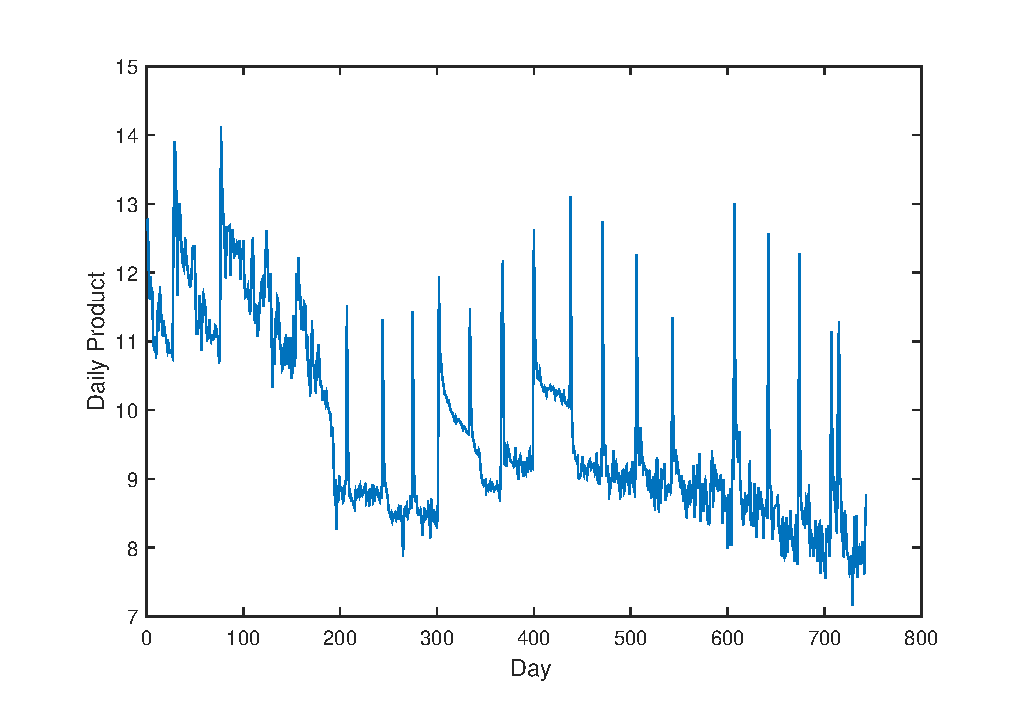
\includegraphics[width=3.5in]{ori-ts}
\caption{The oil production time series.}
\label{figure: oil-production}
\end{figure}

Figure \ref{figure: oil-production} illustrates  the daily production of an oil well for two years, hence there are 730 data points.

Given a time series $T = \{t_i | i = 1, \dots, k+1\}$, the fluctuation from time $i$ to $i + 1$ is given by
\begin{equation}
f_i = \frac{t_{i + 1} - t_i}{t_i},
\end{equation}
where $1 \leq i \leq k+1$.

To model the fluctuation of oil production, we propose the code table as shown in Table \ref{table: code-table}.
Here, the alphabet is $\Sigma$ = \{A, B, C, D, E, F, O, a, b, c, d, e, f\}.
Using $f_i$ and the code table, we can convert $T$ into sequence $S = s_1 s_2 \dots s_k$.
A part of the sequence of the time series in Figure \ref{figure: oil-production} is AcCCAcECeffBeeEedEEEeeDEoBAcdfD.

\begin{table}[h]\caption{The code table}\label{table: code-table}
\centering
\setlength{\tabcolsep}{16pt}
\begin{tabular}{cccccc}
\hline
$f_i$          & Code  & $f_i$               & Code \\
\hline
$(-1\%, 1\%)$  & O\\
$[1\%, 2\%)$   & A     & $(-2\%, -1\%]$      & a\\
$[2\%, 3\%)$   & B     & $(-3\%, -2\%]$      & b\\
$[3\%, 4\%)$   & C     & $(-4\%, -3\%]$      & c\\
$[4\%, 6\%)$   & D     & $(-6\%, -4\%]$      & d\\
$[6\%, 10\%)$  & E     & $(-10\%, -6\%]$     & e\\
$[10\%, +\infty)$ & F     & $(-\infty, -10\%]$   & f\\
\hline
\end{tabular}
\end{table}

Based on the $\Sigma$, we empirically let $\Gamma$ = \{D, d, E, e, F, f\}, $\Lambda$ = \{B, C, b, c\} and $\Omega$ = \{o, a, A\}.
This is because bigger fluctuation is considered more important.
In order to discuss the characteristic of Type I to Type V patterns, we first obtain frequent patterns for each type of pattern.
Second, for Type I to Type V patterns, we choose a pattern with support not less than 3.
Finally, we present the figure of the position matched by the pattern.

\subsubsection{Results}\label{subsection: time-series-results}

\begin{figure}[tbh!]
    \centering
	 \subfigure[boBoD]{
	 \begin{minipage}[t]{0.25\linewidth}
	  \includegraphics[width=1.1in]{TypeI-1}
	  \label{fig:I-1}
	 \end{minipage}
	 }
     \subfigure[booBBaD]{
	 \begin{minipage}[t]{0.25\linewidth}
	  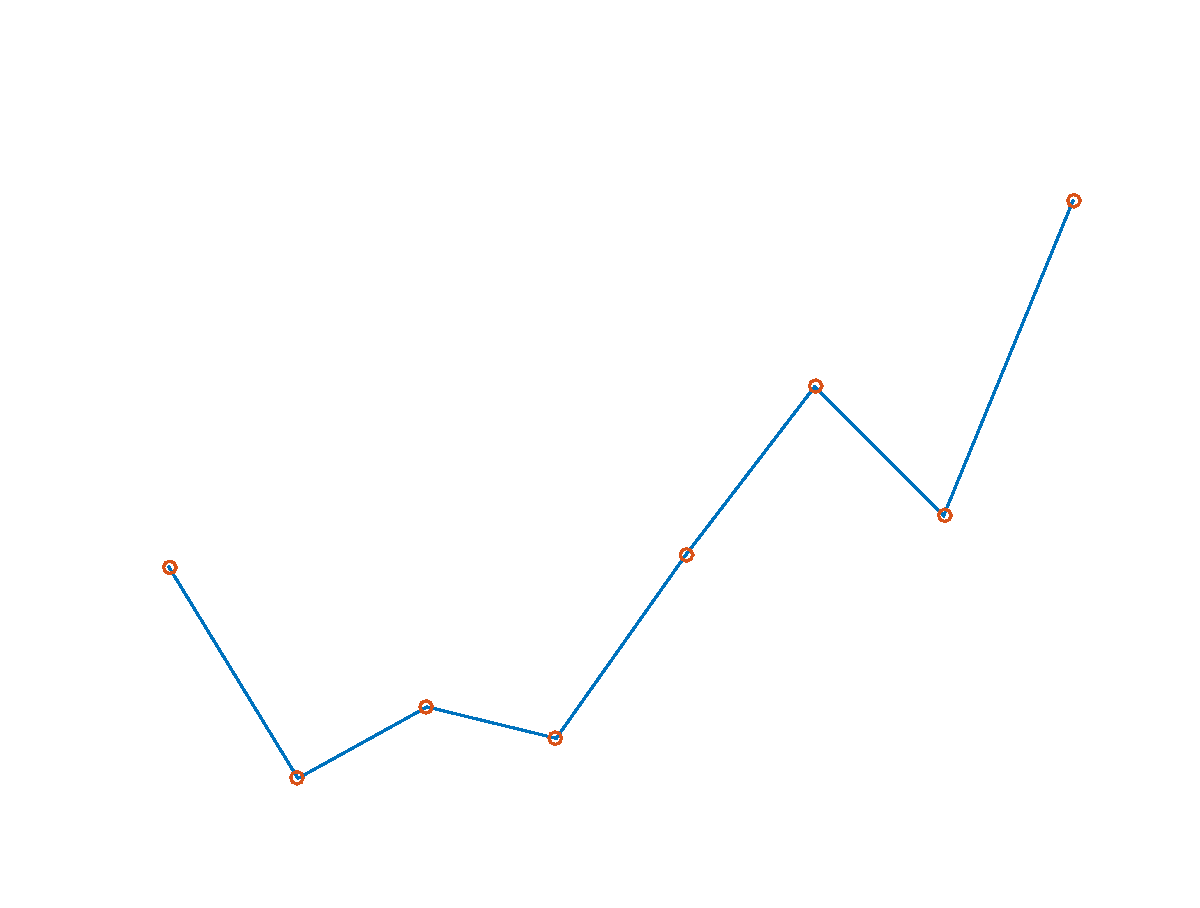
\includegraphics[width=1.1in]{TypeI-2}
	  \label{fig:I-2}
	 \end{minipage}
	 }
     \subfigure[boBAD]{
	 \begin{minipage}[t]{0.25\linewidth}
	  \includegraphics[width=1.1in]{TypeI-3}
	  \label{fig:I-3}
	 \end{minipage}
	 }
	 \subfigure[boB]{
	 \begin{minipage}[t]{0.25\linewidth}
	  \includegraphics[width=1.1in]{TypeII-1}
	  \label{fig:II-1}
	 \end{minipage}
	 }
     \subfigure[boB]{
	 \begin{minipage}[t]{0.25\linewidth}
	  \includegraphics[width=1.1in]{TypeII-2}
	  \label{fig:II-2}
	 \end{minipage}
	 }
     \subfigure[boB]{
	 \begin{minipage}[t]{0.25\linewidth}
	  \includegraphics[width=1.1in]{TypeII-3}
	  \label{fig:II-3}
	 \end{minipage}
	 }
	 \subfigure[ooBaeA]{
	 \begin{minipage}[t]{0.25\linewidth}
	  \includegraphics[width=1.1in]{TypeIII-1}
	  \label{fig:III-1}
	 \end{minipage}
	 }
     \subfigure[oaoaoCA]{
	 \begin{minipage}[t]{0.25\linewidth}
	  \includegraphics[width=1.1in]{TypeIII-2}
	  \label{fig:III-2}
	 \end{minipage}
	 }
     \subfigure[ooBaAAA]{
	 \begin{minipage}[t]{0.25\linewidth}
	  \includegraphics[width=1.1in]{TypeIII-3}
	  \label{fig:III-3}
	 \end{minipage}
	 }
	 \subfigure[aaCDoa]{
	 \begin{minipage}[t]{0.25\linewidth}
	  \includegraphics[width=1.1in]{TypeIV-1}
	  \label{fig:IV-1}
	 \end{minipage}
	 }
     \subfigure[aoDoa]{
	 \begin{minipage}[t]{0.25\linewidth}
	  \includegraphics[width=1.1in]{TypeIV-2}
	  \label{fig:IV-2}
	 \end{minipage}
	 }
     \subfigure[aoDaBa]{
	 \begin{minipage}[t]{0.25\linewidth}
	  \includegraphics[width=1.1in]{TypeIV-3}
	  \label{fig:IV-3}
	 \end{minipage}
	 }
	 \subfigure[eDE]{
	 \begin{minipage}[t]{0.25\linewidth}
	  \includegraphics[width=1.1in]{TypeV-1}
	  \label{fig:V-1}
	 \end{minipage}
	 }
     \subfigure[eDE]{
	 \begin{minipage}[t]{0.25\linewidth}
	  \includegraphics[width=1.1in]{TypeV-2}
	  \label{fig:V-2}
	 \end{minipage}
	 }
     \subfigure[eDCE]{
	 \begin{minipage}[t]{0.25\linewidth}
	  \includegraphics[width=1.1in]{TypeV-3}
	  \label{fig:V-3}
	 \end{minipage}
	 }
	 \caption{Patterns matched for five types, (a-c) match bBD of Type I, (d-f) match boB of Type II,
(g-i) match oaA of Type III, (j-l) match aDa of Type IV, and (m-o) match eDE of Type V.}
	 \label{figure: oil-patterns}
\end{figure}

Figure \ref{figure: oil-patterns} depicts the time series matched by the patterns.
Here we observe that
\begin{enumerate}[1)]
\item{A Type I pattern matches some similar subsequences with minor differences.}
\item{A Type II pattern only matches very similar subsequences.}
\item{A Type III pattern may match some very dissimilar subsequences.}
\item{A Type IV pattern may also match some very dissimilar subsequences.}
\item{A Type V pattern may also ignore some important change, however it is better than Types III and IV.}
\end{enumerate}

\subsection{Faked Chinese text}\label{subsection: text}
Frequent patterns in the text are often viewed as keywords.
Keywords extraction is an interesting direction with many efficient algorithms.
The keywords of texts are often presented in an intuitive way on web pages.

We discuss pattern discovery on faked Chinese text.
Some text creators may want to distribute advertisements on illegal stuff such as faked money or invoice.
They know that the keywords might be mined by a program and consequently, the text will be removed by email or web servers.
Hence they insert some characters into the text, so that the text is still readable for human.
Examples include ``\CJK{GBK}{song}{��a��**��1Ʊ}" (faked invoice)and ``\CJK{GBK}{song}{��@��*��++��}" (faked official seal).
Since different characters are inserted in different positions, a plain text mining algorithms will fail to discover these keywords/patterns.

Our question is: Can our algorithm discover the same keywords when the text is deliberately faked?
For this purpose, we set $\Lambda = \{$\CJK{GBK}{song}{��}, \CJK{GBK}{song}{��}, \CJK{GBK}{song}{��}, \dots\}.
In some situations they are structural auxiliary words.
For example, \CJK{GBK}{song}{��} distinguishes ``mine" from ``I."
In others they express certain meaning.
For example, \CJK{GBK}{song}{��} also stands for ``target."
All other Chinese characters belongs to $\Gamma$.
Latin characters, numbers, and mathematical operators are included in $\Omega$.
That is, $\Omega = \{0, 1, \dots, 9, +, -, *, \dots, a, b, \dots z\}$.
We will randomly insert a small proportion of weak characters and an even smaller proportion of medium characters into the text.
According to Table \ref{table: relationships}, all five types of patterns can be mined using our algorithm.

\subsubsection{Data and parameter settings}\label{subsubsection: chinese-text-data}
\begin{table}[h]\caption{Data for text mining}\label{table: text-data}
\centering
\setlength{\tabcolsep}{20pt}
\begin{tabular}{ccccccl}
\hline
Category           & Quantity       & Length\\
\hline
News               & 5              & 1k \\
Novel              & 5              & 6k-100k \\
History            & 5              & 6k-8k \\
Law                & 10             & 2k-6k \\
\hline
\end{tabular}
\end{table}

As listed in Table \ref{table: text-data}, a total of 25 text files are downloaded from the Internet.
The filed of content includes news, novel, poem and history.
The length ranges from 1k to 100k.

Different proportion of weak characters are inserted into the text.
To control the number of parameters, we set the proportion between inserted medium characters and weak characters to be $\frac{1}{10}$.

\subsubsection{Evaluation measure}\label{subsubsection: chinese-measure}
We undertake the following steps to evaluate the effectiveness of our algorithms.
First, we obtain the top-k frequent plain patterns with length $l$ from the original text.
The set is denoted by $\mathcal{P}_l^o$.
This is done through adjusting the parameter $\rho$ through binary search.
Second, we find out the top-k frequent weak patterns with length $l$ from the faked text.
The set is denoted by $\mathcal{P}_l^f$.
The accuracy of the algorithm for length $l$ is defined as
\begin{equation}\label{equation: text-accuracy}
acc_l = \frac{|\mathcal{P}_l^o \cap \mathcal{P}_l^f|}{|\mathcal{P}_l^o|}.
\end{equation}
To show the validity of the algorithm, frequent plain patterns on the faked text is also mined.
In this way the accuracy of the plain pattern discovery algorithm is obtained.

Here we consider the pattern length while computing the accuracy.
The reason is that a frequency that appropriate for one length would be  quite inappropriate for another.
To obtain a few length-4 patterns, we may set the threshold $\rho$ to be quite low, and the number of length-2 patterns might be overwhelming.
Taking them as a whole will make length-4 patterns quite invisible.

\subsubsection{Results}\label{subsubsection: chinese-results}

\begin{figure}[tbh!]
	 \centering
	 \subfigure[News, length = 2]{
	 \begin{minipage}[c]{2.2in}
	 %\centering
	  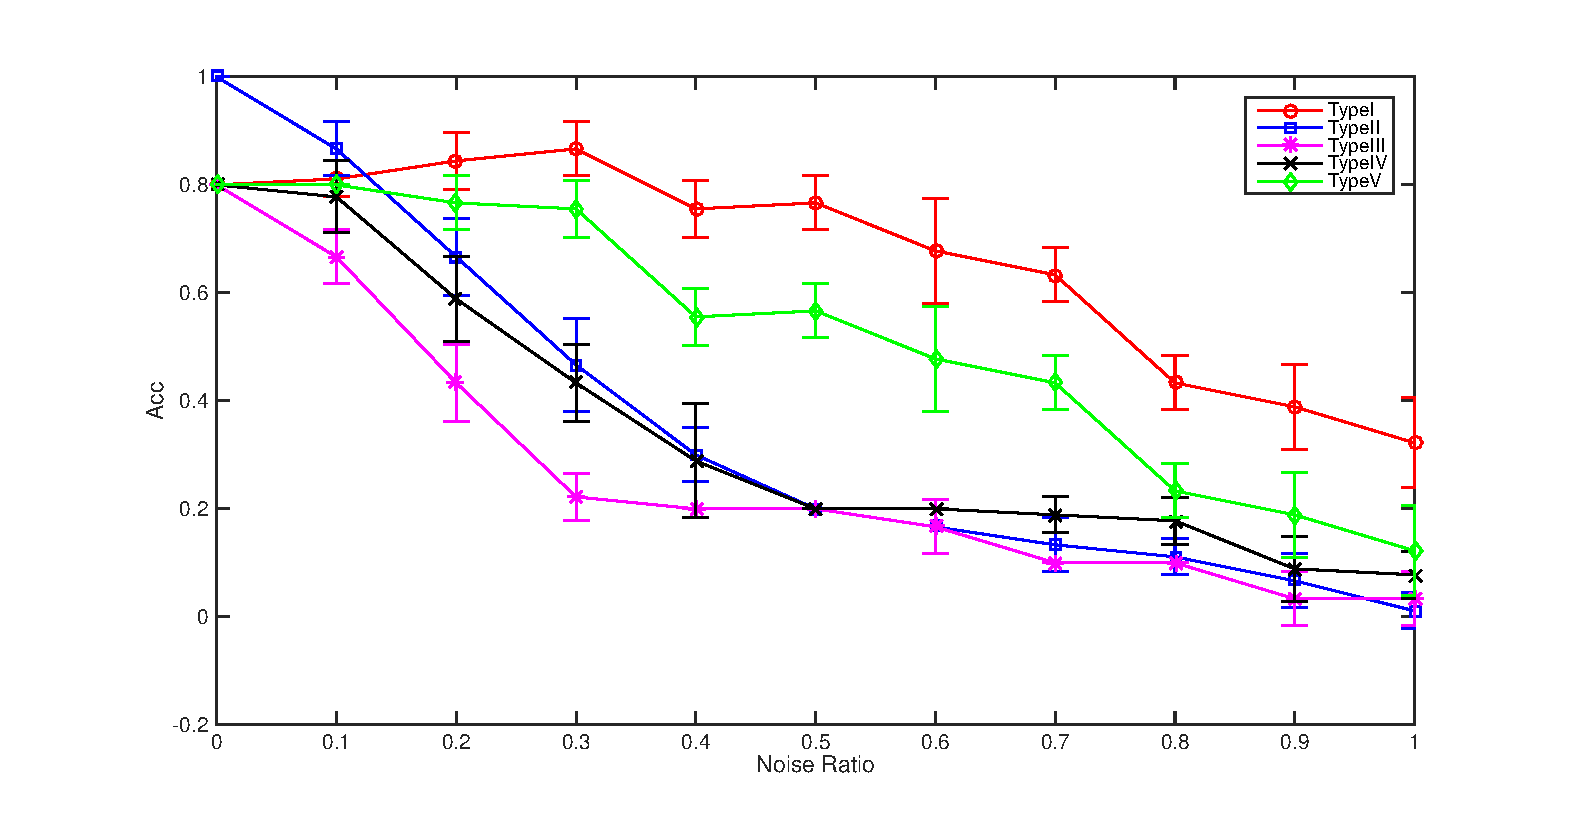
\includegraphics[width=2.2in]{textlength2-news}
	 \end{minipage}
	 }
	 \subfigure[Novel, length = 2]{
     \begin{minipage}[c]{2.2in}
	 %\centering
	  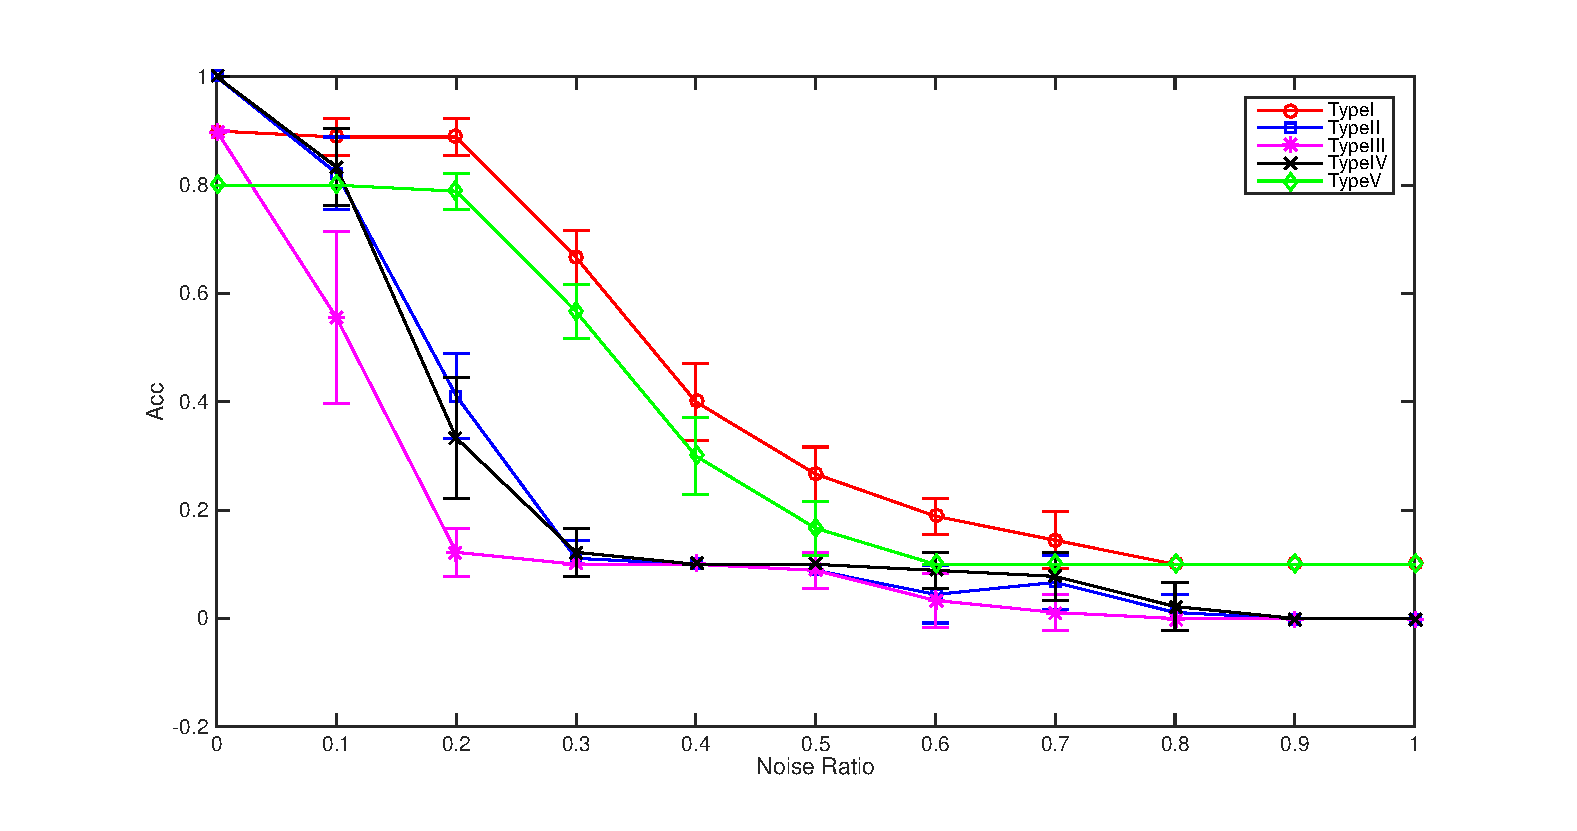
\includegraphics[width=2.2in]{textlength2-novel}
	 \end{minipage}
	 }
	 \subfigure[Law, length = 2]{
	 \begin{minipage}[c]{2.2in}
	 %\centering
	  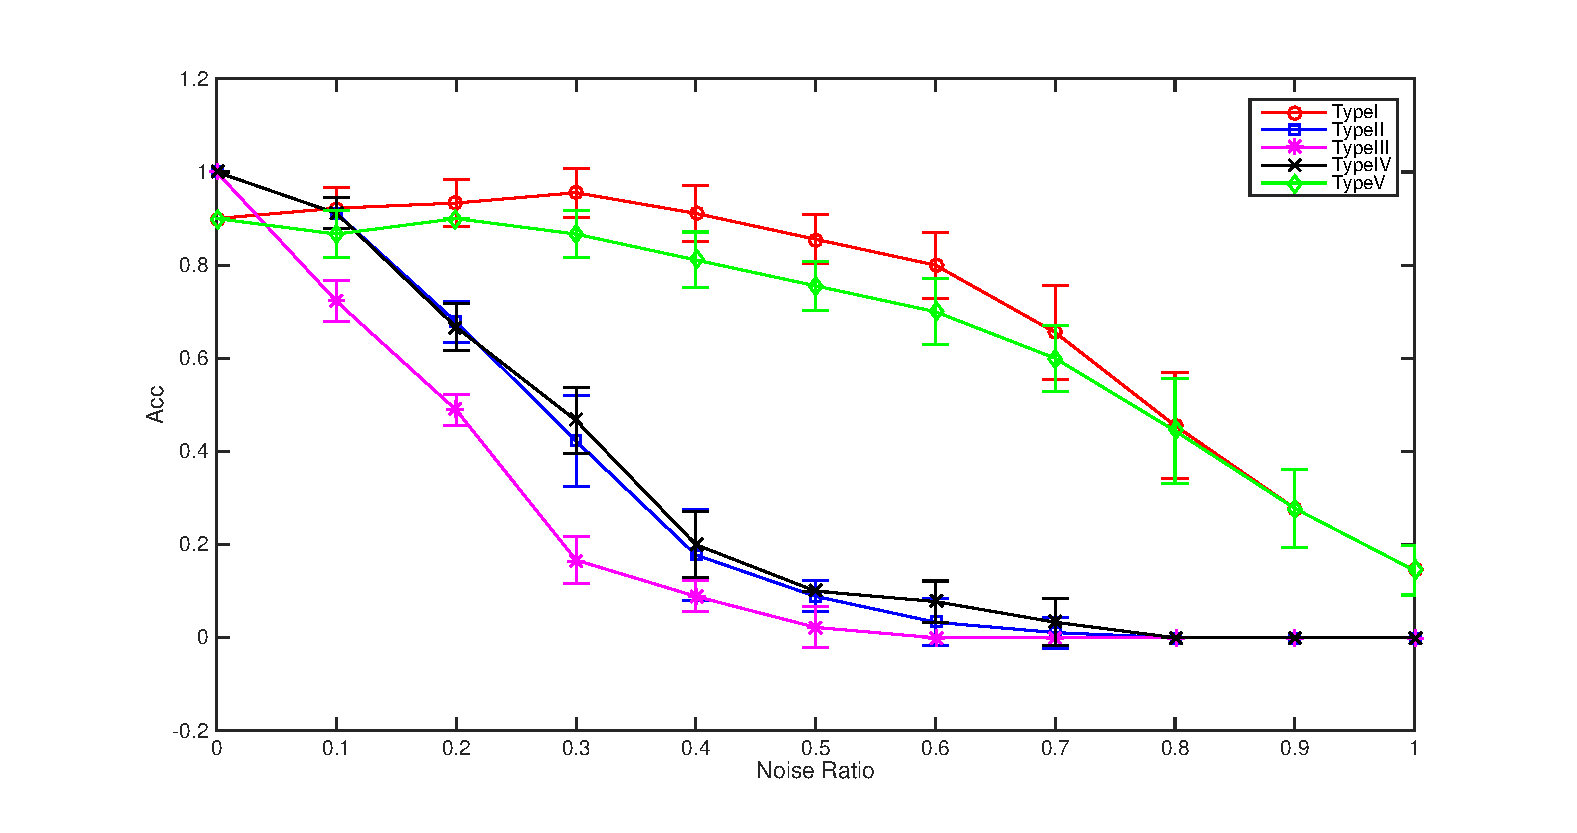
\includegraphics[width=2.2in]{textlength2-law}
	 \end{minipage}
	 }
	 \subfigure[History, length = 2]{
	 \begin{minipage}[c]{2.2in}
	 %\centering
	  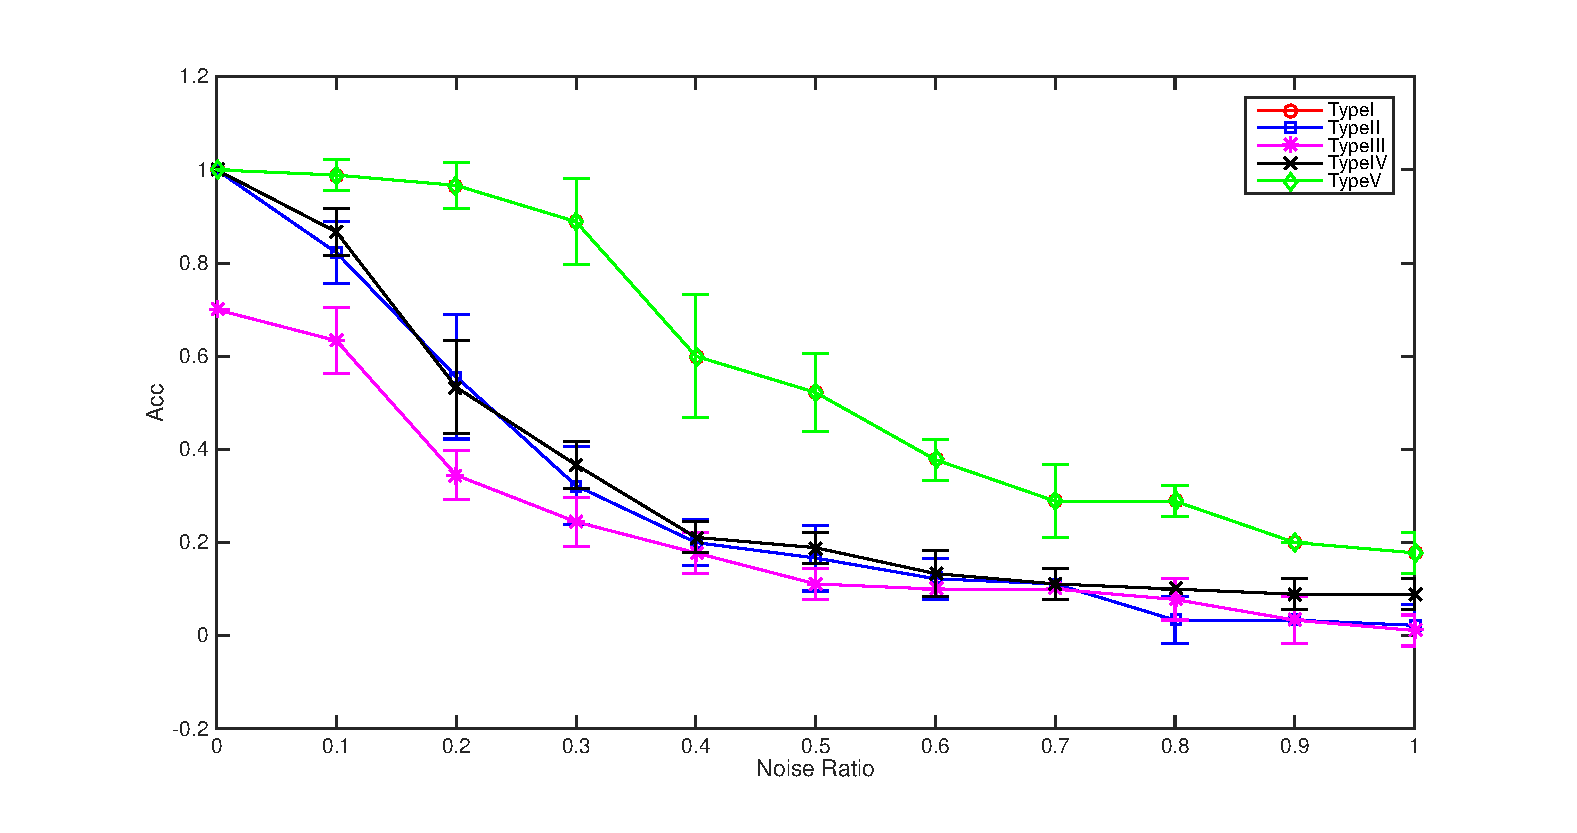
\includegraphics[width=2.2in]{textlength2-history}
	 \end{minipage}
	 }
	 \subfigure[News, length = 3]{
	 \begin{minipage}[c]{2.2in}
	 %\centering
	  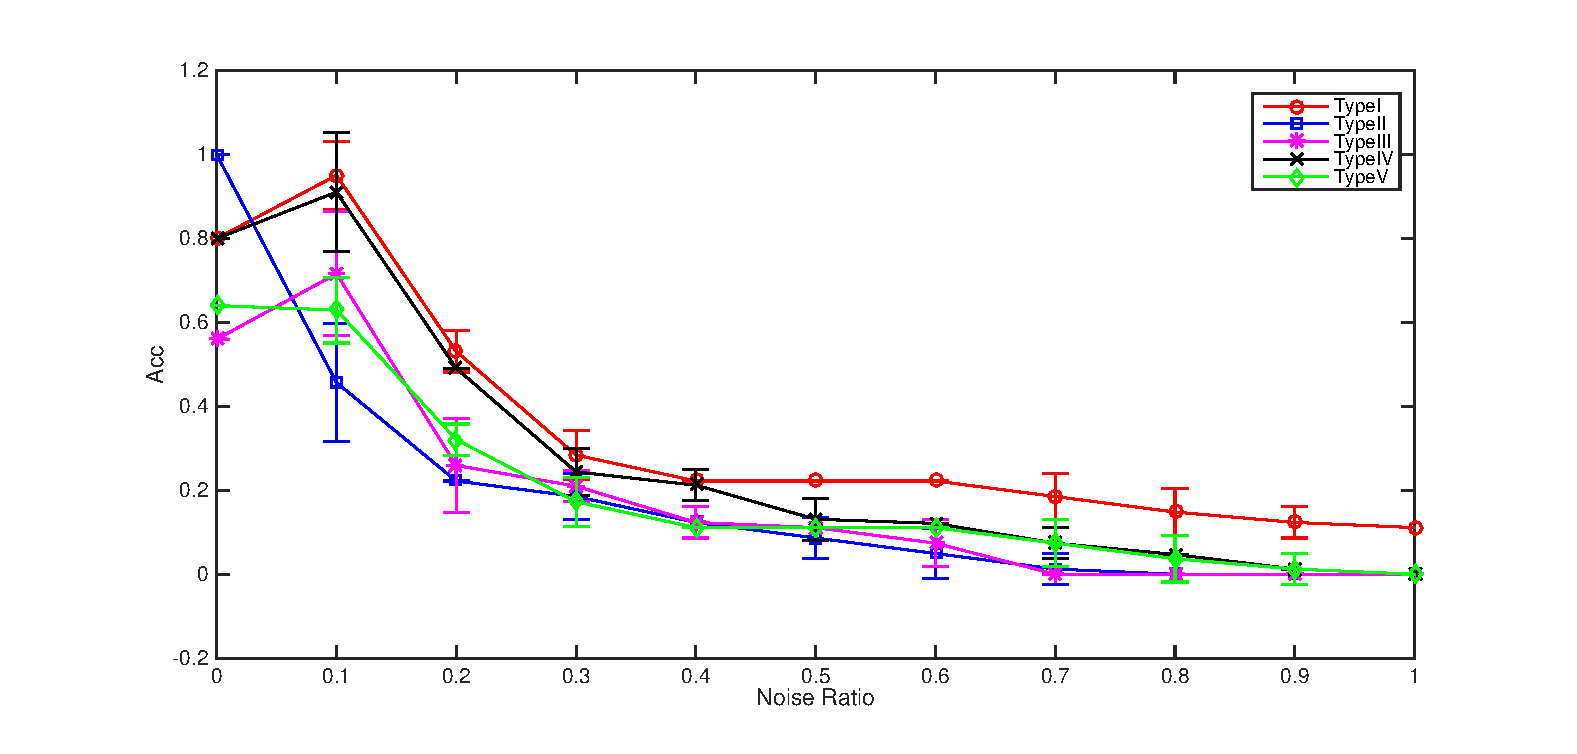
\includegraphics[width=2.2in]{textlength3-news}
	 \end{minipage}
	 }
	 \subfigure[Novel, length = 3]{
     \begin{minipage}[c]{2.2in}
	 %\centering
	  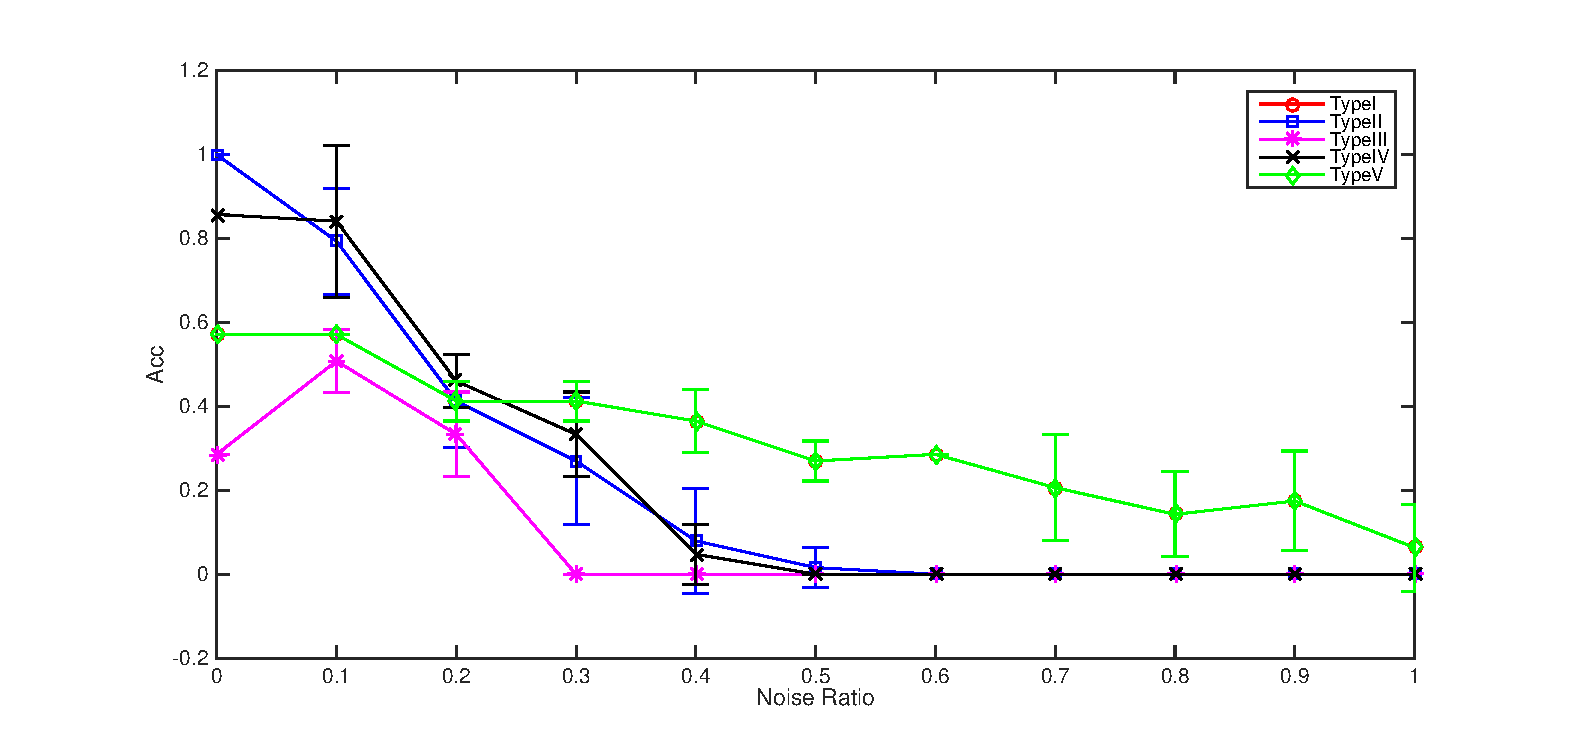
\includegraphics[width=2.2in]{textlength3-novel}
	 \end{minipage}
	 }
	 \subfigure[Law, length = 3]{
	 \begin{minipage}[c]{2.2in}
	 %\centering
	  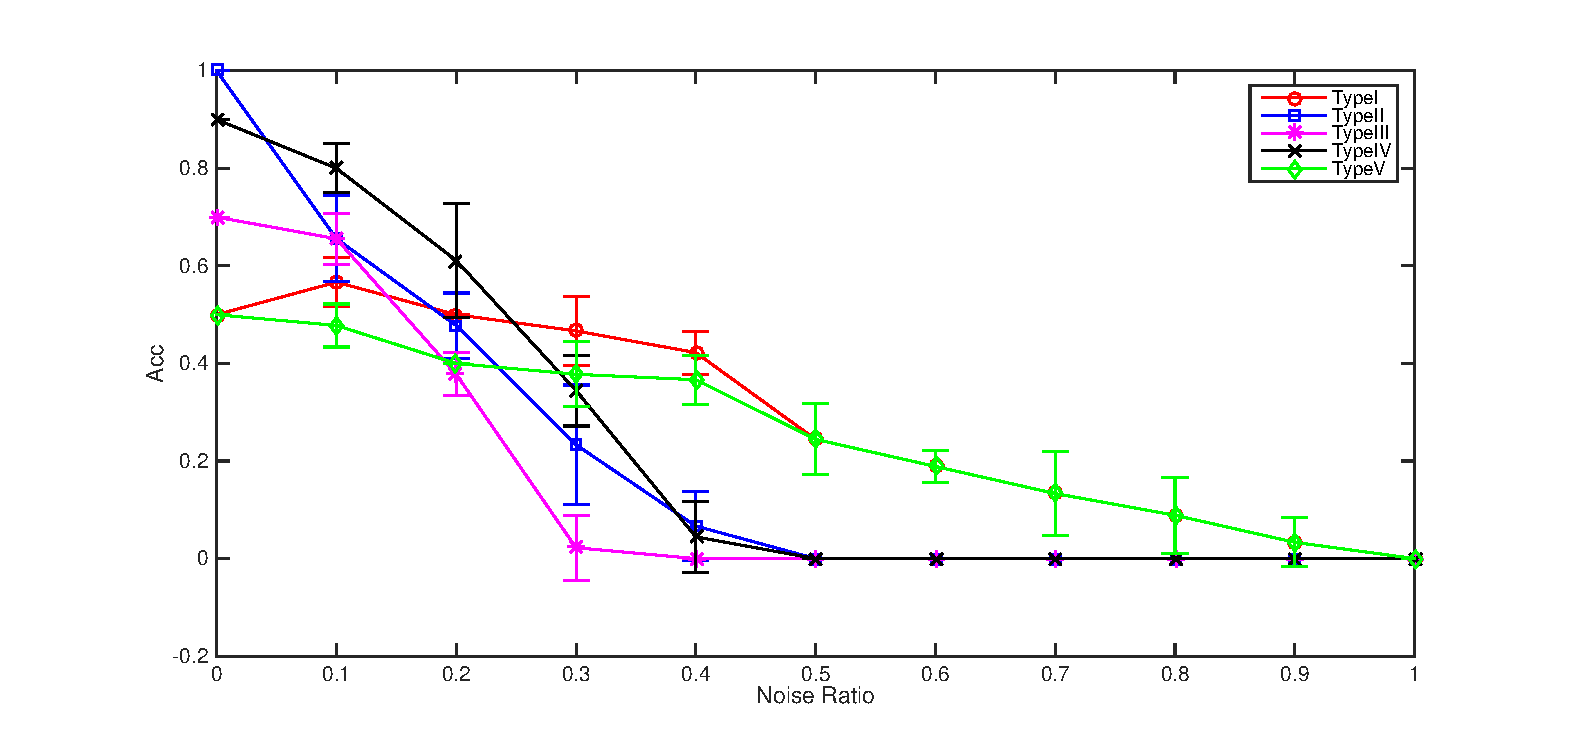
\includegraphics[width=2.2in]{textlength3-law}
	 \end{minipage}
	 }
	 \subfigure[History, length = 3]{
	 \begin{minipage}[c]{2.2in}
	 %\centering
	  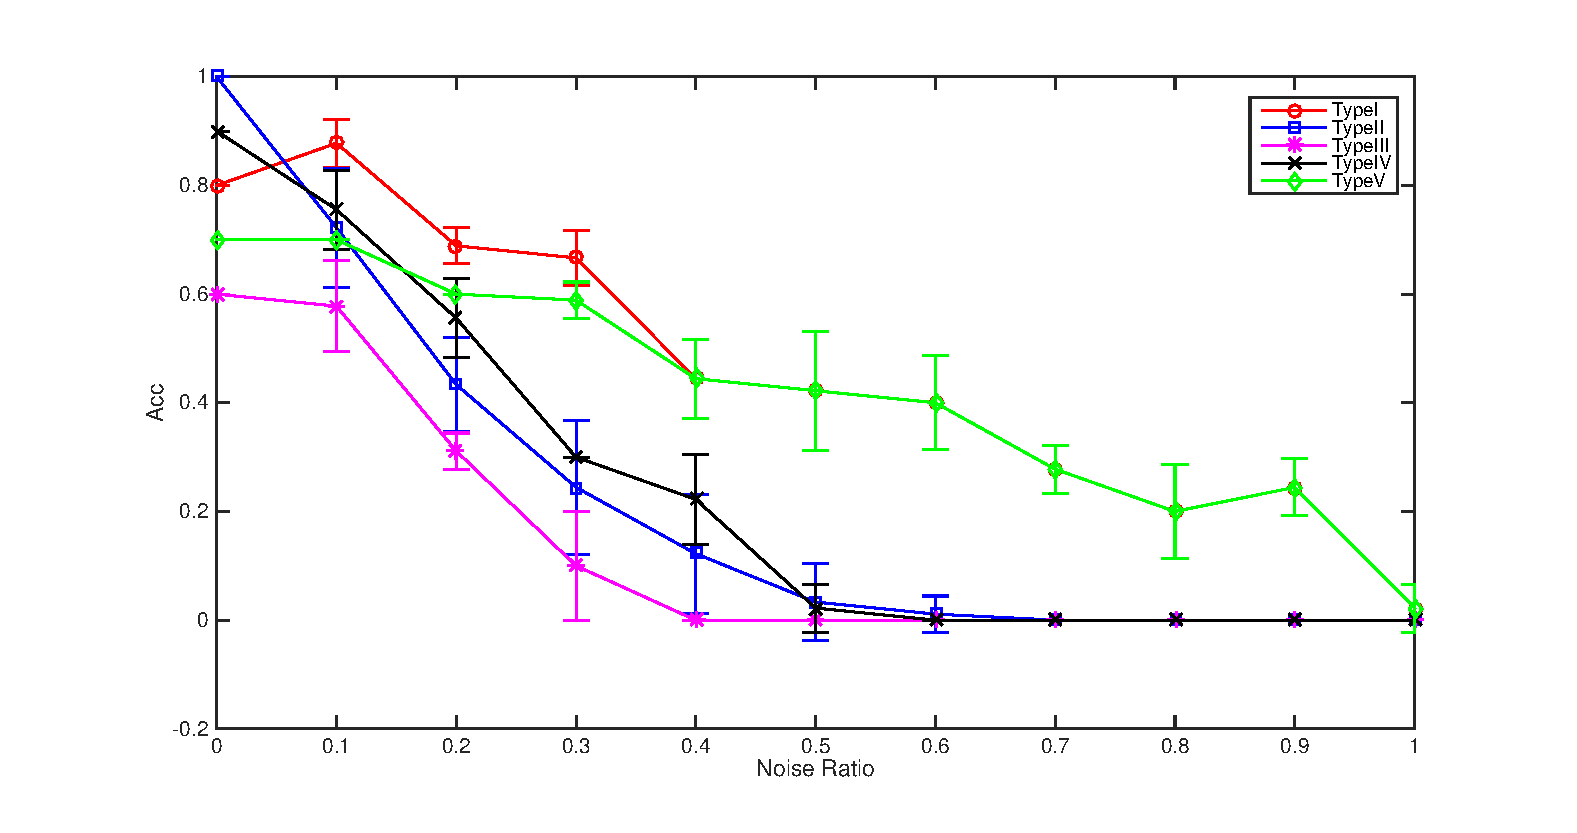
\includegraphics[width=2.2in]{textlength3-history}
	 \end{minipage}
	 }
	 \caption{Accuracy using all five types of patterns with length 2 or 3.}
	 \label{figure: text-acc-length2-3}
\end{figure}

Figure \ref{figure: text-acc-length2-3} presents the results of length 2 and 3 patterns, respectively.
For each text, we generate 10 fake versions, and obtain the mining accuracy on these versions.
Note that the noise ratio can be greater than 1.
In this case there are more inserted text than the original, and the text is badly faked.

Figures \ref{figure: text-acc-length2-3} (a)-(d) illustrate the accuracy of Type I to Type V patterns with length 2 on News, Novel, Law and History Chinese texts.
It can be observed that the Type I performs the best, while Type III performs the worst.
The accuracy of all types of patterns decreases with the increase of the noise ratio.
In Figure \ref{figure: text-acc-length2-3} (d), both Type I and Type V the same best performance.
This is because the most of middle elements in $\Lambda$ are not frequent.
Therefore, the obtained frequent tri-patterns (Type I) do not contain these middle elements.
Hence, Type I patterns are the same as Type V patterns.

Figures \ref{figure: text-acc-length2-3} (e)-(h) illustrate the results with length 3 on these four Chinese texts.
On the News text (Figure \ref{figure: text-acc-length2-3} (e)), Type I is always the best with the noise ratio ranging from 0.1 to 1.0.
When there is no noise (noise ratio = 0.0), Type I and Type IV are the second best one following Type II.
The accuracies of Type I and Type IV are the same as each other and very closet to 0.8.
On the Novel text (Figure \ref{figure: text-acc-length2-3} (f)), Type I and Type V has the same accuracy as each other and perform the best with the noise ratio ranging from 0.3 to 1.0.
When the noise ratio ranging from 0.0 to 0.3, the accuracy of Type I is less than those of Type II and Type IV.
On the Law text (Figure \ref{figure: text-acc-length2-3} (g)), Type I performs the best when the noise ratio ranges from 0.3 to 1.0.
Moreover, from 0.5 to 1.0, the accuracy of Type I is the same as Type V.
On the History text (Figure \ref{figure: text-acc-length2-3} (h)), Type I performs the best when the noise ratio ranges from 0.1 to 1.0.
When the noise ratio is 0.0, Type I performs worse than Type II and Type IV.
However, its accuracy is up to 0.8.

Table \ref{table: text-mining-results} lists the accuracy of different types of patterns on all 25 texts when the noise ratio is 30\% and the pattern length is 2.
We can observe that the accuracy of Type I is always the highest.
For all 25 texts, Type I obtains 8 highest accuracies no less than 0.9.
The lowest one is 0.5, which is still the best one.
Note that, the accuracy of Type V is the same as Type I on some texts (e.g., Law: nsfc.gov.cn).
The reason is that most middle elements in $\Lambda$ are infrequent.

\begin{table}[h]\caption{Results summary of text mining}\label{table: text-mining-results}
\centering
\setlength{\tabcolsep}{1pt}
\scalebox{0.7}{
\begin{tabular}{cccccccccc}
\hline
\multirow{2}{*}{Type} & \multirow{2}{*}{Source}  &  \multicolumn{5}{c}{Accuracy}\\
\cline{3-7}
 & & Type I   & Type II  & Type III  & Type IV  & Type V \\
\hline
\multirow{5}{*}{News}      & news.sohu.com    & $\mathbf{1.0000 \pm 0.0000}$ & $0.5111 \pm 0.1050$  & $0.2000 \pm 0.0866$   & $0.5777 \pm 0.1092$   & $\mathbf{1.0000 \pm 0.0000}$\\

          & finance.ifeng.com   & $\mathbf{0.9111 \pm 0.0333}$  & $0.5777 \pm 0.0833$  & $0.3666 \pm 0.1000$  & $0.6333 \pm 0.1500$   & $\mathbf{0.9111 \pm 0.0333}$\\

          & news.china.com  & $\mathbf{0.6555 \pm 0.0527}$ & $0.4111 \pm 0.0600$   & $0.2222 \pm 0.0440$  & $0.4333 \pm 0.0499$   & $0.5555 \pm 0.0527$\\

          & chinanews.com   & $\mathbf{0.9666 \pm 0.0499}$ & $0.5333 \pm 0.1118$   & $0.3000 \pm 0.1118$  & $0.5666 \pm 0.099$     & $\mathbf{0.9666 \pm 0.0499}$\\

          & dvdc100.com   & $\mathbf{0.8777 \pm 0.0440}$ & $0.4888 \pm 0.1054$  & $0.2222 \pm 0.0440$   & $0.3888 \pm 0.1054$ & $0.7222 \pm 0.0666$\\
\cline{2-7}
\multirow{5}{*}{Novel}     & jjwxc.net   & $\mathbf{0.7000 \pm 0.0866}$ & $0.1777 \pm 0.0666$   & $0.0999 \pm 0.0001$ & $0.1222 \pm 0.0440$    & $0.6000 \pm 0.0866$\\

          & xs8.cn   & $\mathbf{0.7000 \pm 0.0001}$ & $0.4333 \pm 0.0001$   & $0.3777 \pm 0.0440$  & $0.4111 \pm 0.0333$  & $\mathbf{0.7000 \pm 0.0001}$\\

          & xs8.cn  & $\mathbf{0.8777 \pm 0.0440}$ & $0.3333 \pm 0.0707$   & $0.0666 \pm 0.050$  & $0.3333 \pm 0.0500$    & $0.7888 \pm 0.0333$\\

          & xs8.cn   & $\mathbf{0.6333 \pm 0.0499}$ & $0.2555 \pm 0.0726$    & $0.099 \pm 0.0001$  & $0.2777 \pm 0.0440$   & $\mathbf{0.6333 \pm 0.0499}$\\

          & news.ifeng.com   & $\mathbf{0.5777 \pm 0.0440}$ & $0.2222 \pm 0.0440$    & $0.1999 \pm 0.0001$ & $0.1999 \pm 0.0001$   & $\mathbf{0.5777 \pm 0.0440}$\\
\cline{2-7}
\multirow{5}{*}{Law}       & law-lib.com   & $\mathbf{0.9000 \pm 0.0001}$ & $0.3333 \pm 0.0500$ & $0.1888 \pm 0.0781$  & $0.3555 \pm 0.0527$   & $0.7000 \pm 0.0001$\\

          & nsfc.gov.cn   & $\mathbf{0.9888 \pm 0.0333}$ & $0.7888 \pm 0.0927$   & $0.4777 \pm 0.0666$  & $0.8777 \pm 0.0440$ & $\mathbf{0.9888 \pm 0.0333}$\\

          & gov.cn   & $\mathbf{0.9444 \pm 0.0527}$ & $0.4111 \pm 0.0600$    & $0.1555 \pm 0.0527$ & $0.4555 \pm 0.0527$    & $0.8555 \pm 0.0527$\\

          & jincao.com  & $\mathbf{0.8888 \pm 0.0333}$ & $0.3111 \pm 0.0333$  & $0.1666 \pm 0.0500$   & $0.3111 \pm 0.0333$    & $0.7999 \pm 0.0001$\\

          & bj.xinhuanet.com   & $\mathbf{0.9888 \pm 0.0333}$ & $0.5111 \pm 0.0333$   & $0.3888 \pm 0.0600$  & $0.5666 \pm 0.0499$    & $0.9000 \pm 0.0010$\\
\cline{2-7}
\multirow{5}{*}{History}   & news.ifeng.com   & $\mathbf{0.5000 \pm 0.0001}$ & $0.2333 \pm 0.0499$  & $0.1888 \pm 0.0333$ & $0.2111 \pm 0.0333$    & $\mathbf{0.5000 \pm 0.0001}$\\
          & news.ifeng.com   & $\mathbf{0.9222 \pm 0.0666}$ & $0.3888 \pm 0.0781$   & $0.2222 \pm 0.0440$ & $0.3999 \pm 0.0500$    & $\mathbf{0.9222 \pm 0.0666}$\\

          & 71.cn   & $\mathbf{0.7000 \pm 0.0001}$ & $0.2444 \pm 0.1013$    & $0.0999 \pm 0.0001$  & $0.2111 \pm 0.0781$  & $\mathbf{0.7000 \pm 0.0001}$\\

          & news.ifeng.com  & $\mathbf{0.7000 \pm 0.0001}$ & $0.3333 \pm 0.0500$  & $0.1666 \pm 0.0500$  & $0.3000 \pm 0.0500 $   & $\mathbf{0.7000 \pm 0.0001}$\\

          &  news.ifeng.com  & $\mathbf{1.0000 \pm 0.0000}$ & $0.3888 \pm 0.0600$   & $0.2444 \pm 0.0527$   & $0.3888 \pm 0.0333$   & $\mathbf{1.0000 \pm 0.0000}$\\
\hline
\end{tabular}
}
\end{table}

The answer to our question is: when the text is slightly faked (e.g., less than 30\% characters are inserted), most original keywords can be still mined with Type I patterns through our algorithms.
We also observe that
\begin{enumerate}[1)]
\item{Type I patterns are the most accurate among all five types.}
\item{Type I patterns are always more accurate than Type V patterns.}
\item{Type III patterns are most sensitive to noise.
    There are often plenty of frequent but meaningless patterns.
    The reason lies in that any character can form the pattern, while they can also be ignored.}
\item{From Figures \ref{figure: text-acc-length2-3}, when the noise ratio is low, some Type IV patterns are causal, making Type IV patterns less accurate than Type II ones.
    However, with the increase of the noise ratio, Type IV patterns gradually outperforms Type II ones.}
\end{enumerate}

%
%%%%%%%%%%%%%%%%%%%%%%%%%%%%%%%%%%
% beginning of a new section
%%%%%%%%%%%%%%%%%%%%%%%%%%%%%%%%%%
%
\section{Conclusions}\label{section: conclusions}
In this paper, we defined a frequent tri-pattern discovered from a tri-partition alphabet.
Existing sequential patterns (Type II through V) are special cases of our tri-pattern.
Hence the proposed TPM algorithm can also discover all other types by only changing the tri-partition strategy and/or the wildcard gap.
Experiments on protein sequence, time series and Chinese texts show that:
\begin{enumerate}[1)]
\item{Type I patterns provide a better tradeoff between flexibility and accuracy than the other four.}
\item{The proposed algorithm can obtain frequent tri-patterns effectively and reliably.}
\end{enumerate}

The following research topics deserve further investigation:
\begin{enumerate}[1)]
\item{Pattern explanation and evaluation involving domain-specific experts. For some real applications such as oil-well production pattern discovery, the meaning of the pattern can be only evaluated by experts.}
\item{Application of the discovered patterns. These patterns can be used to not only reveal the situation or status of the sequence, but also cluster sequences or prediction.}
\item{Tri-pattern discovery from multiple time series, which is more complex, and more widely exists in reality.}
\end{enumerate}

We hope that this work opens a new door for the development of three-way decision.

%
%%%%%%%%%%%%%%%%%%%%%%%%%%%%%%%%%%
% beginning of a new section
%%%%%%%%%%%%%%%%%%%%%%%%%%%%%%%%%%
%
\section*{Acknowledgements}\label{section: acknowledgements}
This work is in part supported by National Science Foundation of China [grant numbers 61379089, 41604114]; and the Open Research Fund of Sichuan Key Laboratory for Nature Gas and Geology [grant number 2015trqdz04].

% references section
%\section*{References}\label{section: References}

%\bibliographystyle{elsarticle-num-names}
\bibliographystyle{elsart-num-sort}
%\bibliographystyle{model1c-num-names}
\bibliography{bibitems/trialphabet,bibitems/relatedworks}

\end{document}
